\chapter[Fuentes equivalentes potenciadas por el gradiente]{
    Fuentes equivalentes potenciadas por el gradiente
}
\chaptermark{Fuentes equiv. potenciadas por el gradiente}
\label{cha:eql-gradient-boosted}

Este capítulo es una traducción al español del artículo titulado
\emph{Gradient-boosted equivalent sources} escrito por Santiago R. Soler
y Leonardo Uieda, y publicado en \emph{Geophysical Journal
International} en Agosto de 2021 \citep{soler2021}.
Una preimpresión del artículo se encuentra disponible bajo licencia Creative
Commons Atribución 4.0 Internacional en
\href{https://eartharxiv.org/}{EarthArXiv} (doi:
\href{https://doi.org/10.31223/X58G7C}{10.31223/X58G7C}).


% Import files with parameter values generated by notebooks
\newcommand{\AustraliaSmallAreaEastingSize}{$300 \, \text{km}$}
\newcommand{\AustraliaSmallAreaNorthingSize}{$300 \, \text{km}$}
\newcommand{\AustraliaSmallAreaNPoints}{14934}
\newcommand{\AustraliaDepthMin}{$1000 \, \text{m}$}
\newcommand{\AustraliaDepthMax}{$15000 \, \text{m}$}
\newcommand{\AustraliaDampingMin}{0.01}
\newcommand{\AustraliaDampingMax}{10000}
\newcommand{\AustraliaEqlDepth}{$3000 \, \text{m}$}
\newcommand{\AustraliaEqlDamping}{100}
\newcommand{\AustraliaEqlSpacing}{$1800 \, \text{m}$}
\newcommand{\AustraliaEqlWindowSize}{$225 \, \text{km}$}
\newcommand{\AustraliaEqlRmsScore}{$1.33 \, \text{mGal}$}
\newcommand{\AustraliaEqlNSources}{796744}
\newcommand{\AustraliaEqlGridNLongitude}{2442}
\newcommand{\AustraliaEqlGridNLatitude}{2085}
\newcommand{\AustraliaEqlGridHeight}{$2127.58 \, \text{m}$}\newcommand{\BestAirborneSourceBelowDataConstantDepthDamping}{10$^{-2}$}
\newcommand{\BestAirborneSourceBelowDataConstantDepthDepth}{7000}
\newcommand{\BestAirborneSourceBelowDataConstantDepthRms}{0.35}
\newcommand{\BestAirborneSourceBelowDataConstantDepthNPoints}{5673}
\newcommand{\BestAirborneSourceBelowDataRelativeDepthDamping}{10$^{-2}$}
\newcommand{\BestAirborneSourceBelowDataRelativeDepthDepth}{9000}
\newcommand{\BestAirborneSourceBelowDataRelativeDepthRms}{0.35}
\newcommand{\BestAirborneSourceBelowDataRelativeDepthNPoints}{5673}
\newcommand{\BestAirborneSourceBelowDataVariableDepthDamping}{1}
\newcommand{\BestAirborneSourceBelowDataVariableDepthDepthFactor}{1}
\newcommand{\BestAirborneSourceBelowDataVariableDepthDepth}{1450}
\newcommand{\BestAirborneSourceBelowDataVariableDepthKNearest}{15}
\newcommand{\BestAirborneSourceBelowDataVariableDepthRms}{0.36}
\newcommand{\BestAirborneSourceBelowDataVariableDepthNPoints}{5673}
\newcommand{\BestAirborneBlockAveragedSourcesConstantDepthDamping}{10$^{-4}$}
\newcommand{\BestAirborneBlockAveragedSourcesConstantDepthDepth}{9000}
\newcommand{\BestAirborneBlockAveragedSourcesConstantDepthSpacing}{3000}
\newcommand{\BestAirborneBlockAveragedSourcesConstantDepthRms}{0.34}
\newcommand{\BestAirborneBlockAveragedSourcesConstantDepthNPoints}{1100}
\newcommand{\BestAirborneBlockAveragedSourcesRelativeDepthDamping}{10$^{-3}$}
\newcommand{\BestAirborneBlockAveragedSourcesRelativeDepthDepth}{9000}
\newcommand{\BestAirborneBlockAveragedSourcesRelativeDepthSpacing}{2000}
\newcommand{\BestAirborneBlockAveragedSourcesRelativeDepthRms}{0.34}
\newcommand{\BestAirborneBlockAveragedSourcesRelativeDepthNPoints}{1663}
\newcommand{\BestAirborneBlockAveragedSourcesVariableDepthDamping}{10$^{-2}$}
\newcommand{\BestAirborneBlockAveragedSourcesVariableDepthSpacing}{2000}
\newcommand{\BestAirborneBlockAveragedSourcesVariableDepthDepthFactor}{2}
\newcommand{\BestAirborneBlockAveragedSourcesVariableDepthDepth}{50}
\newcommand{\BestAirborneBlockAveragedSourcesVariableDepthKNearest}{15}
\newcommand{\BestAirborneBlockAveragedSourcesVariableDepthRms}{0.33}
\newcommand{\BestAirborneBlockAveragedSourcesVariableDepthNPoints}{1663}
\newcommand{\BestAirborneGridSourcesConstantDepthDamping}{10$^{-1}$}
\newcommand{\BestAirborneGridSourcesConstantDepthDepth}{7000}
\newcommand{\BestAirborneGridSourcesConstantDepthSpacing}{1000}
\newcommand{\BestAirborneGridSourcesConstantDepthRms}{0.34}
\newcommand{\BestAirborneGridSourcesConstantDepthNPoints}{12544}\newcommand{\BestGroundSourceBelowDataConstantDepthDamping}{10$^{-1}$}
\newcommand{\BestGroundSourceBelowDataConstantDepthDepth}{7000}
\newcommand{\BestGroundSourceBelowDataConstantDepthRms}{0.78}
\newcommand{\BestGroundSourceBelowDataConstantDepthNPoints}{963}
\newcommand{\BestGroundSourceBelowDataRelativeDepthDamping}{10$^{-1}$}
\newcommand{\BestGroundSourceBelowDataRelativeDepthDepth}{9000}
\newcommand{\BestGroundSourceBelowDataRelativeDepthRms}{0.79}
\newcommand{\BestGroundSourceBelowDataRelativeDepthNPoints}{963}
\newcommand{\BestGroundSourceBelowDataVariableDepthDamping}{1}
\newcommand{\BestGroundSourceBelowDataVariableDepthDepthFactor}{1}
\newcommand{\BestGroundSourceBelowDataVariableDepthDepth}{1000}
\newcommand{\BestGroundSourceBelowDataVariableDepthKNearest}{15}
\newcommand{\BestGroundSourceBelowDataVariableDepthRms}{0.80}
\newcommand{\BestGroundSourceBelowDataVariableDepthNPoints}{963}
\newcommand{\BestGroundBlockAveragedSourcesConstantDepthDamping}{10$^{-1}$}
\newcommand{\BestGroundBlockAveragedSourcesConstantDepthDepth}{7000}
\newcommand{\BestGroundBlockAveragedSourcesConstantDepthSpacing}{3000}
\newcommand{\BestGroundBlockAveragedSourcesConstantDepthRms}{0.77}
\newcommand{\BestGroundBlockAveragedSourcesConstantDepthNPoints}{518}
\newcommand{\BestGroundBlockAveragedSourcesRelativeDepthDamping}{10$^{-1}$}
\newcommand{\BestGroundBlockAveragedSourcesRelativeDepthDepth}{7000}
\newcommand{\BestGroundBlockAveragedSourcesRelativeDepthSpacing}{3000}
\newcommand{\BestGroundBlockAveragedSourcesRelativeDepthRms}{0.79}
\newcommand{\BestGroundBlockAveragedSourcesRelativeDepthNPoints}{518}
\newcommand{\BestGroundBlockAveragedSourcesVariableDepthDamping}{10$^{-1}$}
\newcommand{\BestGroundBlockAveragedSourcesVariableDepthSpacing}{3000}
\newcommand{\BestGroundBlockAveragedSourcesVariableDepthDepthFactor}{1}
\newcommand{\BestGroundBlockAveragedSourcesVariableDepthDepth}{600}
\newcommand{\BestGroundBlockAveragedSourcesVariableDepthKNearest}{15}
\newcommand{\BestGroundBlockAveragedSourcesVariableDepthRms}{0.72}
\newcommand{\BestGroundBlockAveragedSourcesVariableDepthNPoints}{518}
\newcommand{\BestGroundGridSourcesConstantDepthDamping}{10$^{2}$}
\newcommand{\BestGroundGridSourcesConstantDepthDepth}{3000}
\newcommand{\BestGroundGridSourcesConstantDepthSpacing}{2000}
\newcommand{\BestGroundGridSourcesConstantDepthRms}{0.97}
\newcommand{\BestGroundGridSourcesConstantDepthNPoints}{3192}\newcommand{\BoostOverlappingWindowSize}{$30000 \, \text{m}$}\newcommand{\EqlBoostAirborneRmsScore}{$0.38 \, \text{mGal}$}
\newcommand{\EqlBoostAirborneDepth}{$3000 \, \text{m}$}
\newcommand{\EqlBoostAirborneDamping}{0.1}
\newcommand{\EqlBoostAirborneSpacing}{$2 \, \text{km}$}
\newcommand{\EqlBoostAirborneWindowSize}{$20 \, \text{km}$}
\newcommand{\EqlBoostAirborneNSources}{1663}
\newcommand{\EqlBoostAirborneMinDepth}{$1000 \, \text{m}$}
\newcommand{\EqlBoostAirborneMaxDepth}{$19000 \, \text{m}$}
\newcommand{\EqlBoostAirborneMinDamping}{1e-06}
\newcommand{\EqlBoostAirborneMaxDamping}{10}\newcommand{\AirborneSourceBelowDataConstantDepthDamping}{10$^{-4}$, 10$^{-3}$,$\dots$, 10$^{2}$}
\newcommand{\AirborneSourceBelowDataConstantDepthDepth}{1000 to 17000, step size 2000}
\newcommand{\AirborneSourceBelowDataRelativeDepthDamping}{10$^{-4}$, 10$^{-3}$,$\dots$, 10$^{2}$}
\newcommand{\AirborneSourceBelowDataRelativeDepthDepth}{1000 to 17000, step size 2000}
\newcommand{\AirborneSourceBelowDataVariableDepthDamping}{10$^{-4}$, 10$^{-3}$,$\dots$, 10$^{2}$}
\newcommand{\AirborneSourceBelowDataVariableDepthDepthFactor}{1 to 6, step size 1}
\newcommand{\AirborneSourceBelowDataVariableDepthDepth}{50 to 1450, step size 200}
\newcommand{\AirborneSourceBelowDataVariableDepthKNearest}{1, 5, 10 and 15}
\newcommand{\AirborneBlockAveragedSourcesConstantDepthDamping}{10$^{-4}$, 10$^{-3}$,$\dots$, 10$^{2}$}
\newcommand{\AirborneBlockAveragedSourcesConstantDepthDepth}{1000 to 17000, step size 2000}
\newcommand{\AirborneBlockAveragedSourcesConstantDepthSpacing}{1000, 2000, 3000 and 4000}
\newcommand{\AirborneBlockAveragedSourcesRelativeDepthDamping}{10$^{-4}$, 10$^{-3}$,$\dots$, 10$^{2}$}
\newcommand{\AirborneBlockAveragedSourcesRelativeDepthDepth}{1000 to 17000, step size 2000}
\newcommand{\AirborneBlockAveragedSourcesRelativeDepthSpacing}{1000, 2000, 3000 and 4000}
\newcommand{\AirborneBlockAveragedSourcesVariableDepthDamping}{10$^{-4}$, 10$^{-3}$,$\dots$, 10$^{2}$}
\newcommand{\AirborneBlockAveragedSourcesVariableDepthSpacing}{1000, 2000, 3000 and 4000}
\newcommand{\AirborneBlockAveragedSourcesVariableDepthDepthFactor}{1 to 6, step size 1}
\newcommand{\AirborneBlockAveragedSourcesVariableDepthDepth}{50 to 1450, step size 200}
\newcommand{\AirborneBlockAveragedSourcesVariableDepthKNearest}{1, 5, 10 and 15}
\newcommand{\AirborneGridSourcesConstantDepthDamping}{10$^{-3}$, 10$^{-2}$,$\dots$, 10$^{2}$}
\newcommand{\AirborneGridSourcesConstantDepthDepth}{1000 to 9000, step size 2000}
\newcommand{\AirborneGridSourcesConstantDepthSpacing}{1000, 2000 and 3000}\newcommand{\GroundSourceBelowDataConstantDepthDamping}{10$^{-4}$, 10$^{-3}$,$\dots$, 10$^{2}$}
\newcommand{\GroundSourceBelowDataConstantDepthDepth}{1000 to 17000, step size 2000}
\newcommand{\GroundSourceBelowDataRelativeDepthDamping}{10$^{-4}$, 10$^{-3}$,$\dots$, 10$^{2}$}
\newcommand{\GroundSourceBelowDataRelativeDepthDepth}{1000 to 17000, step size 2000}
\newcommand{\GroundSourceBelowDataVariableDepthDamping}{10$^{-4}$, 10$^{-3}$,$\dots$, 10$^{2}$}
\newcommand{\GroundSourceBelowDataVariableDepthDepthFactor}{0.1, 0.5, 1, 2, 3, 4, 5 and 6}
\newcommand{\GroundSourceBelowDataVariableDepthDepth}{0 to 1400, step size 200}
\newcommand{\GroundSourceBelowDataVariableDepthKNearest}{1, 5, 10 and 15}
\newcommand{\GroundBlockAveragedSourcesConstantDepthDamping}{10$^{-4}$, 10$^{-3}$,$\dots$, 10$^{2}$}
\newcommand{\GroundBlockAveragedSourcesConstantDepthDepth}{1000 to 17000, step size 2000}
\newcommand{\GroundBlockAveragedSourcesConstantDepthSpacing}{1000, 2000, 3000 and 4000}
\newcommand{\GroundBlockAveragedSourcesRelativeDepthDamping}{10$^{-4}$, 10$^{-3}$,$\dots$, 10$^{2}$}
\newcommand{\GroundBlockAveragedSourcesRelativeDepthDepth}{1000 to 17000, step size 2000}
\newcommand{\GroundBlockAveragedSourcesRelativeDepthSpacing}{1000, 2000, 3000 and 4000}
\newcommand{\GroundBlockAveragedSourcesVariableDepthDamping}{10$^{-4}$, 10$^{-3}$,$\dots$, 10$^{2}$}
\newcommand{\GroundBlockAveragedSourcesVariableDepthSpacing}{1000, 2000, 3000 and 4000}
\newcommand{\GroundBlockAveragedSourcesVariableDepthDepthFactor}{0.1, 0.5, 1, 2, 3, 4, 5 and 6}
\newcommand{\GroundBlockAveragedSourcesVariableDepthDepth}{0 to 1400, step size 200}
\newcommand{\GroundBlockAveragedSourcesVariableDepthKNearest}{1, 5, 10 and 15}
\newcommand{\GroundGridSourcesConstantDepthDamping}{10$^{1}$, 10$^{2}$, 10$^{3}$ and 10$^{4}$}
\newcommand{\GroundGridSourcesConstantDepthDepth}{1000 to 9000, step size 2000}
\newcommand{\GroundGridSourcesConstantDepthSpacing}{1000, 2000, 3000 and 4000}\newcommand{\SourceLayoutsSchematicsObservations}{166}
\newcommand{\SourceLayoutsSchematicsSourceBelowData}{166}
\newcommand{\SourceLayoutsSchematicsGridSources}{378}
\newcommand{\SourceLayoutsSchematicsBlockAveragedSources}{87}\newcommand{\NPrisms}{64}
\newcommand{\ModelEasting}{$111319 \, \text{m}$}
\newcommand{\ModelNorthing}{$111319 \, \text{m}$}
\newcommand{\ModelDepth}{$10000 \, \text{m}$}
\newcommand{\ModelMinDensity}{$-900 \, \text{kg} \, \text{m}^{-3}$}
\newcommand{\ModelMaxDensity}{$500 \, \text{kg} \, \text{m}^{-3}$}
\newcommand{\SurveyEasting}{$111319 \, \text{m}$}
\newcommand{\SurveyNorthing}{$110576 \, \text{m}$}
\newcommand{\SurveyNoise}{$1 \, \text{mGal}$}
\newcommand{\GroundSurveyPoints}{963}
\newcommand{\GroundSurveyMinHeight}{$0 \, \text{m}$}
\newcommand{\GroundSurveyMaxHeight}{$2052.2 \, \text{m}$}
\newcommand{\AirborneSurveyPoints}{5673}
\newcommand{\AirborneSurveyMinHeight}{$359 \, \text{m}$}
\newcommand{\AirborneSurveyMaxHeight}{$1255 \, \text{m}$}
\newcommand{\TargetHeight}{$2000 \, \text{m}$}
\newcommand{\TargetSpacing}{$2 \, \text{km}$}
\newcommand{\TargetEastingSize}{57}
\newcommand{\TargetNorthingSize}{56}


\section{Introducción}

Las mediciones de las anomalías en los campos potenciales, como el disturbio de
gravedad o anomalías magnéticas, son ampliamente utilizadas en la exploración
geofísica debido a su bajo costo de adquisición.
Estos datos pueden ser recolectados utilizando sistemas terrestres, aéreos,
marítimos o satelitales.
Durante las mediciones terrestres, los datos son recabados siguiendo
trayectorias irregulares a lo largo de la superficie del terreno, produciendo
altas variaciones en la altitud de los puntos de observación en zonas
montañosas.
Las metodologías aéreas y satelitales obtienen los datos a lo largo de líneas
de vuelo, produciendo mediciones muy próximas espacialmente a lo largo de
trayectorias casi rectas, pero con espaciados mucho mayores entre líneas
adyacentes.
La altitud de observación también puede variar en estos casos debido al
movimiento vertical de la aeronave.
El procesado de estos datos suele incluir interpolaciones sobre grillas
regulares a altitudes constante, tanto para mejorar la visualización con el
objetivo de realizar interpretaciones, así como para preparar los datos para
posteriores procesados y/o modelado (por ejemplo, reducción al polo, cálculo de
derivadas, continuación ascendente, deconvolución de Euler).

Existen muchos métodos en la literatura para realizar interpolaciones en dos
dimensiones, por ejemplo splines de curvatura continua en tensión
\citep{smith1990}, splines biharmónicas (placa delgada) \citep{sandwell1987},
y kriging \citep{hansen1993}.
Estos métodos de propósito general poseen limitaciones a la hora de interpolar
datos provenientes de campos potenciales:
(i)~no son capaces de tomar en cuenta las altitudes de los puntos de
observación,
(ii)~las funciones interpoladoras no son necesariamente harmónicas, siendo esta
la principal presuposición de muchas técnicas de procesado (por ejemplo,
continuación ascendente y derivadas verticales).

Un método ampliamente utilizado para interpolar datos gravitatorios
y magnéticos es la técnica de fuentes equivalentes (también conocida como capa
equivalente -\emph{equivalent layer} en inglés-, funciones de bases radiales
-\emph{radial basis functions} en inglés-, o interpolaciones con funciones de
Green).
Inicialmente introducida por \citet{dampney1969}, el método consiste en ajustar
un modelo de finitas fuentes elementales a los datos observados, y luego usar
ese modelo para predecir nuevos valores.
Además de las interpolaciones, las fuentes equivalentes han sido utilizadas
para realizar reducciones al polo de datos magnéticos \citep{silva1986,
nakatsuka2006, guspi2009}, continuación ascendente \citep{emilia1973, li2010},
procesado conjunto de datos del gradiente gravimétrico \citet{barnes2011},
modelado del campo magnético litosférico \citep{kother2015}, recuperación del
vector de inducción magnética a partir de anomalías magnéticas de campo total
\citep{li2020}, entre otras.

Vale nombrar también el método de colocación por mínimos cuadrados
(\emph{least-squares collocation method} en inglés), ampliamente utilizado en
geodesia.
\citep[][y referencias allí citadas]{tscherning2015}.
Esta metodología se suele aplicar para combinar e interpolar diferentes
funciones lineales de anomalías derivadas del potencial gravitatorio (anomalías
de gravedad, disturbio de gravedad, deflexiones de la vertical, altitud del
geoide, etc.).
Al igual que las fuentes equivalentes, el método de colocación requiere
resolver un sistema lineal grande, cuyo orden equivale a la cantidad de datos
observados.
De esta manera, la aplicación práctica de ambos métodos sufren de los mismos
desafíos computacionales.

Muchas variantes de la técnica de fuentes equivalentes han sido propuestas,
usualmente intentando obtener soluciones más precisas o en menor tiempo.
Los factores claves que varían entre ellos son: (i) el tipo de fuente, (ii) la
ubicación de las fuentes, y (iii) la estrategia de solución.

Los tipos de fuentes más utilizados son masas puntuales para datos
gravitatorios o dipolos para datos magnéticos \citep[e.g.,~][]{vonfrese1981,
silva1986, mendonca1994, siqueira2017}.
Sin embargo, también se han utilizado exitosamente prismas rectangulares
\citep[por~ej.,][]{barnes2011, jirigalatu2019, li2020} y tesseroides
\citep{bouman2016}.
De hecho, incluso fuentes puntuales en conjunto con funciones simple como la
inversa de la distancia, en vez del campo gravitatorio o magnético, pueden ser
utilizadas como fuentes equivalentes \citep{cordell1992}.

La ubicación de las fuentes suele elegirse de acuerdo a alguno de las
siguientes estrategias.
El método más común es distribuir las fuentes en una grilla regular a una
profundad constante \citep[por~ej.,~][]{leao1989, barnes2011, oliveira2013}.
Alternativamente, podemos ubicar una fuente debajo de cada punto de observación
\citep[por~ej.,~][]{cordell1992, siqueira2017}.
Algunos trabajos recientes de \citet{li2020} ubican las fuentes en dos capas
superpuestas a profundidades diferentes.

Los coeficientes de las fuentes equivalentes suelen ser estimados mediante
mínimos cuadrados ponderados.
Esto implica una carga computacional alta cuando la cantidad de datos es grande
(por ej. muestras aéreas o satelitales).
Para reducir la carga computacional, \citet{mendonca1994} construyen la
solución iterativamente al tratar un solo dato al mismo tiempo utilizando el
concepto de \emph{dato equivalente}.

\citet{leao1989} procesan los datos de entrada mediante una ventana móvil, solo
ajustando los datos dentro de la ventan y prediciendo las observaciones en su
centro.
\citet{li2010} y \citet{barnes2011} aplican diferentes operaciones para generar
una representación dispersa de la matriz de sensibilidades (\emph{wavelet
compression} y \emph{quadtree discretization}, respectivamente), lo cual mejora
significativamente la velocidad de ejecución del algoritmo de mínimos
cuadrados.
\citet{oliveira2013} parametrizan las fuentes equivalentes como una función
polinomial bivariada a trazos, reduciendo el número de parámetros en la
solución.
\citet{siqueira2017} desarrollaron una solución iterativa en la cual la matriz
de sensibilidades es transformada en una matriz diagonal con términos
constantes a través del concepto de \emph{exceso de masa}.
\citet{jirigalatu2019} aplican el método Gauss-FFT para acelerar las
operaciones vinculadas al modelado directo y resuelven el problema de mínimos
cuadrados utilizando el descenso del gradiente con el objetivo de evitar
calcular las matrices Hessianas y resolver sistemas lineales.


Muchos de los métodos existentes resuelven problemas subdeterminados,
requiriendo un número mayor de fuentes equivalentes que de cantidad de datos.
Algunos de ellos alcanzan mayores eficiencias al
restringir su aplicación a tipos de datos específicos \citep{siqueira2017},
realizar las interpolaciones sobre grillas regulares \citep{leao1989},
o requieren datos ya grillados \citep{takahashi2020},
por nombrar algunos.
Además, muchas de las optimizaciones propuestas son complejas de implementar en
un programa de computación, limitando que sean ampliamente utilizados.

En el presente trabajo, proponemos dos estrategias para reducir el costo
computacional de la técnica de fuentes equivalentes:

\begin{enumerate}
    \item Reducir el número de fuentes equivalentes para muestras con
        sobremuestreo mediante una estrategia de \emph{promedio en
        bloques} (\emph{block-averaging} en inglés), manteniendo la calidad de
        la solución.
    \item Ajustar el modelo de fuentes equivalentes iterativamente sobre
        ventanas solapadas utilizando un algoritmo de \emph{potenciación del
        gradiente} (\emph{gradient-boosting} en inglés) \citep{friedman2001}.
\end{enumerate}

La primera estrategia consiste en dividir el área de estudio en bloques
y asignar una única fuente a cada bloque, localizada en la ubicación media de
los puntos de datos.
Para muestras aéreas, navales y satelitales, las cuales presentan sobremuestreo
a lo largo de la trayectoria del vehículo, esto puede reducir considerablemente
el tamaño del problema inverso manteniendo a su vez la misma calidad en la
interpolación.

El algoritmo de \emph{potenciación del gradiente} permite ajustar el modelo de
fuentes equivalentes de manera iterativa, operando de manera individual sobre
cada una de las ventanas con solapamiento.
Como resultado, nuestro método resuelve muchos problemas de mínimos cuadrados
de menor tamaño en vez de un único gran problema.
Este posee algunas semejanzas con la estrategia utilizada por \citet{leao1989},
pero sin el requerimiento de que tanto las fuentes como los puntos de
interpolación se encuentren en grillas regulares.

Mediantes pruebas sobre datos sintéticos, mostramos que:
(i)~las fuentes \emph{promediadas en bloque} son capaces de alcanzar el mismo
nivel de precisión que otras disposiciones de fuentes equivalentes más
tradicionales, utilizando una fracción del número de fuentes; y
(ii)~el algoritmo \emph{potenciación del gradiente} reduce significativamente la
memoria necesaria para ajustar grandes cantidades de datos, sin sacrificar
precisión en las predicciones.
Finalmente, una combinación de ambas estrategias es utilizada para procesar una
colección de aproximadamente 1.7 millones de datos de gravedad tomados sobre la
superficie de Australia.

%%%%%%%%%%%%%%%%%%%%%%%%%%%%%%%%%%%%%%%%%%%%%%%%%%%%%%%%%%%%%%%%%%%%%%%%%%%%%%%

\section{Metodología}

\subsection{La técnica de fuentes equivalentes}

De aquí en más seguiremos las \emph{fuentes equivalentes generalizadas}
propuestas por \citet{cordell1992}
y asumiremos que cualquier función harmónica $d(\mathbf{p})$
puede ser aproximada por la suma de los efectos de $M$ fuentes puntuales

\begin{equation}
    d(\mathbf{p})
    =
    \sum\limits_{j=1}^{M} \frac{c_j}{| \mathbf{p} - \mathbf{q}_j
    |} \ ,
    \label{eq:eql-forward}
\end{equation}

\noindent donde $\mathbf{p}$ y $\mathbf{q}_j$ son, respectivamente, los
vectores posición de datos y fuentes en un espacio cartesiano tridimensional,
y $c_j$ es un coeficiente escalar relacionado con la masa puntual localizada en
$\mathbf{q}_j$.
En la sección~\ref{sec:source_distribution} realizamos una discusión acerca de
la distribución horizontal y vertical de las fuentes.

En caso de que poseamos mediciones de nuestra función harmónica en $N$ puntos
de observación
$\{\mathbf{p}_1\ \mathbf{p}_2\ \ldots\ \mathbf{p}_N\}$,
podemos escribir un sistema de $N$ ecuaciones de la forma:

\begin{equation}
    d_i
    =
    \sum\limits_{j=1}^{M} \frac{c_j}{| \mathbf{p}_i - \mathbf{q}_j
    |}
    \quad \forall i=1,2,\ldots,N
    \ ,
    \label{eq:forward-sum}
\end{equation}

\noindent donde $d_i$ es el efecto de las fuentes sobre el punto $\mathbf{p}_i$.
Estas ecuaciones pueden ser expresadas de forma matricial como:

\begin{equation}
    \mathbf{d} = \mathbf{A} \mathbf{c} \ ,
    \label{eq:linear-problem}
\end{equation}

\noindent donde $\mathbf{d}$ es un vector columna que contiene los $N$ valores
predichos sobre cada punto de observación,
$\mathbf{c}$ es un vector columna formado por los $M$ coeficientes $c_j$ y
$\mathbf{A}$ es la matriz Jacobiana de $N \times M$ elementos,
los cuales se definen como:

\begin{equation}
    a_{ij} = \frac{1}{|\mathbf{p}_i - \mathbf{q}_j|}
\end{equation}

Para un conjunto de $N$ observaciones $\mathbf{d}^o$, podemos hallar la
solución de la ecuación~\ref{eq:linear-problem} mediante mínimos cuadrados y de
esa manera obtener los valores de
$\mathbf{c}$ que mejor ajustan a las observaciones.
Estos coeficientes pueden ser, a su vez, utilizados para predecir los valores
de la función harmónica en cualquier otro punto externo a las fuentes,
evaluando la ecuación~\ref{eq:eql-forward}.
El grillado o la continuación ascendente puede entonces ser realizados mediante
predicciones sobre puntos de una grilla regular o sobre puntos a diferentes
altitudes, respectivamente.


\subsection{Solución por mínimos cuadrados amortiguados}
\label{sec:eql_inversion}

Es posible obtener los valores de los coeficientes $\mathbf{c}$ que mejor
ajustan a los valores observados $\mathbf{d}^o$ minimizando la función objetivo

\begin{equation}
    \phi(\mathbf{c}) =
    \left[\mathbf{d}^o - \mathbf{A}\mathbf{c}\right]\trans
    \mathbf{W}
    \left[\mathbf{d}^o - \mathbf{A}\mathbf{c}\right]
    + \lambda_d\ \mathbf{c}\trans\mathbf{c}
    \ ,
    \label{eq:misfit-unscaled}
\end{equation}

\noindent donde
$\mathbf{W}$ es una matriz diagonal de $N \times N$ elementos que contiene los
pesos ponderados de los datos observados, y
$\lambda_d$ es el parámetro de \emph{amortiguamiento} (\emph{damping} en
inglés), mayor que cero y con las mismas unidades que los elementos de la
matriz Jacobiana.

El segundo término del miembro derecho de la ecuación~\ref{eq:misfit-unscaled}
consiste en una regularización Thikhonov de orden cero \citep{tikhonov1977},
también conocida como regularización de amortiguamiento (\emph{damping
regularization}), que se utiliza para estabilizar la solución.

El parámetro de amortiguamiento controla cuánta regularización será aplicada.
Un valor muy grande generaría soluciones muy suaves que fallarían en reproducir
las componentes de altas frecuencias presente en los datos, mientras que un
valor muy pequeño resultaría en un sobreajuste, produciendo resultados de
interpolación irreales
\citep{martinez2016}.
El rango de valores aceptables para el parámetro de amortiguamiento
$\lambda_d$ dependerá de los valores de la matriz Jacobiana $\mathbf{A}$
y de los coeficientes.
Por lo tanto, este rango puede variar (considerablemente en muchas ocasiones)
entre diferentes conjuntos de datos, haciendo difícil una apropiada elección en
la práctica.

Para resolver esta problema, primero escalaremos la matriz Jacobiana de forma
tal que sus elementos sean adimensionales y que cada columna posea varianza
unitaria.
Definimos la matriz diagonal $\mathbf{S}$ como:

\begin{equation}
    \mathbf{S} =
    \begin{bmatrix}
      \sigma_1 & 0 & \cdots &0 \\
      0 & \sigma_2 & \cdots &0 \\
      \vdots & \vdots & \ddots & \vdots \\
      0  & 0 & \cdots & \sigma_M
    \end{bmatrix}_{M \times M}
    ,
\end{equation}

\noindent donde $\sigma_j$ es la desviación estándar de la columna $j$-ésima
de la matriz $\mathbf{A}$.
Luego reescribimos el problema directo de la ecuación~\ref{eq:linear-problem}
como:

\begin{equation}
    \mathbf{d}
    =
    \mathbf{A} \mathbf{S}\inv \mathbf{S} \mathbf{c}
    =
    \Big[
        \mathbf{A} \mathbf{S}\inv
    \Big]
    \Big[
        \mathbf{S} \mathbf{c}
    \Big]
    =
    \mathbf{B} \mathbf{m}
\end{equation}

\noindent donde $\mathbf{B} = \mathbf{A} \mathbf{S}\inv$ es la matriz Jacobiana
escalda y adimensional, y
$\mathbf{m} = \mathbf{S} \mathbf{c}$ es el vector que contiene los coeficientes
escalados cuyas unidades son las mismas que la de los datos.

La función objetivo definida en la ecuación~\ref{eq:misfit-unscaled} puede ser
reescrita como:

\begin{equation}
    \phi(\mathbf{m}) =
    \left[\mathbf{d}^o - \mathbf{B}\mathbf{m}\right]\trans
    \mathbf{W}
    \left[\mathbf{d}^o - \mathbf{B}\mathbf{m}\right]
    + \lambda\ \mathbf{m}\trans\mathbf{m}
    \ ,
    \label{eq:misfit}
\end{equation}

\noindent donde $\lambda$ es un parámetro de \emph{amortiguamiento
adimensional} y la regularización es aplicada a los coeficientes escalados
$\mathbf{m}$ en vez de al vector $\mathbf{c}$.
Utilizando un parámetro de amortiguamiento adimensional nos permite limitar el
rango de valores de $\lambda$ que generan las predicciones más precisas,
independientemente del set de datos y sus unidades.
A partir de nuestra experiencia, recomendamos buscar valores de $\lambda$ entre
$10^{-6}$ y $10^{4}$ variando por orden de magnitud.
La elección del amortiguamiento y de otros hiperparámetros, como la profundidad
de las fuentes, puede realizarse a través de métodos estadísticos conocidos,
como la validación cruzada.

El vector de coeficientes escalados $\hat{\mathbf{m}}$ que minimiza la función
objetivo puede hallarse resolviendo el \emph{sistema de ecuaciones normales}
\citep{menke1989}:

\begin{equation}
    \left[
      \mathbf{B}\trans \mathbf{W} \mathbf{B} + \lambda \mathbf{I}
    \right]
    \hat{\mathbf{m}} =
    \mathbf{B}\trans\mathbf{W}
    \mathbf{d}^o.
    \label{eq:least_squares_solution}
\end{equation}

Una vez que los coeficientes escalados son obtenidos, los coeficientes sin
escalar
$\hat{\mathbf{c}}$ pueden ser calculados quitando el factor de escalado:

\begin{equation}
    \hat{\mathbf{c}} = \mathbf{S}\inv \hat{\mathbf{m}} \ .
\end{equation}

\noindent Las operaciones relacionadas al modelado directo que se utilizan para
realizar predicciones (por ejemplo, interpolaciones seguidas de continuaciones
ascendentes) permanecen sin variaciones al utilizar el vector
$\hat{\mathbf{c}}$ en vez de $\hat{\mathbf{m}}$.


\subsection{Potenciación del gradiente}

La potenciación del gradiente fue inicialmente introducida por
\citet{friedman2001, friedman2002} como un método para ajustar modelos
paramétricos de manera aditiva de la siguiente forma:

\begin{equation}
    d = \sum_{k=1}^K \alpha_k f(\mathbf{c}_k),
\end{equation}

\noindent donde $\alpha_k$ es un coeficiente llamado \emph{tamaño de paso}
y $f$ es una función del vector de parámetros $\mathbf{c}_k$.
Para problemas lineales, estos modelos aditivos pueden expresarse según la
siguiente ecuación matricial:

\begin{equation}
    \mathbf{d} = \sum_{k=1}^K \mathbf{A}_k \mathbf{c}_k \ .
    \label{eq:gb-linear-model}
\end{equation}

\noindent Dada la linealidad de la funciones $f(\mathbf{c}_k)$, los parámetros
de tamaño de paso $\alpha_k$ pueden ser incluidos en el vector de parámetros
$\mathbf{c}_k$.

Aplicando esta técnica al problema de fuentes equivalentes, podemos transformar
la ecuación~\ref{eq:linear-problem} en un modelo aditivo siguiendo estos
pasos:

\begin{enumerate}
  \item Definir un conjunto de $M$ fuentes equivalentes distribuidas a lo
      largo de la zona de estudio (ver sección~\ref{sec:source_distribution}
      para más detalles).
  \item Definir un conjunto de $K$ ventanas solapadas de igual tamaño que
      cubren toda la zona de estudio.
  \item Crear $K$ conjuntos distintos de fuentes equivalentes, uno por cada
      ventana.
      Cada conjunto estará conformado por la proción de las $M$ fuentes
      originales que caen dentro de la respectiva ventana.
      Dado que las ventanas se solapan, el número total de fuentes considerando
      cada uno de los conjuntos será mayor que $M$.
  \item Definir el vector $\mathbf{c}_k$ como los $M_k$ coeficientes
      correspondientes a las fuentes equivalentes de la ventana $k$-ésima.
  \item Definir la matriz $\mathbf{A}_k$ como la matriz Jacobiana de $N \times
      M_k$ elementos entre las fuentes de la ventana $k$-ésima y todos los $N$
      puntos de datos de la muestra.
  \item Modelar los datos predichos por las fuentes como una superposición de
      los efectos de los $K$ conjuntos de fuentes equivalentes
      (ec.~\ref{eq:gb-linear-model}).
\end{enumerate}

El algoritmo de potenciación del gradiente funciona ajustando cada componente
del modelo aditivo, una a la vez, a los residuos de la componente anterior.
\citet{friedman2001} demuestra que esto corresponde a una optimización por
descenso del gradiente en el \emph{espacio funcional}.
El Algoritmo~\ref{alg:gradient_boosting} presenta nuestra adaptación del
algoritmo de potenciación del gradiente para hallar las soluciones  de los $K$
vectores de parámetros $\mathbf{c}_k$ de la ec~\ref{eq:gb-linear-model}
mediante mínimos cuadrados amortiguados.

\begin{algorithm}[!h]
  \DontPrintSemicolon
  \setstretch{1.5}
  Definir el vector residual $\mathbf{r}_{0} = \mathbf{d}^o$ \;
  \For{ $k = 1$ \KwTo $K$ }{


      Calcular la matriz Jacobiana $\mathbf{A}_k$ de $N \times M_k$ elementos
      \;

      $\mathbf{B}_k = \mathbf{A}_k \mathbf{S}_k\inv$
      \nllabel{alg:scale}
      \;

      $
       \hat{\mathbf{m}}_k = \left[\mathbf{B}_k\trans \mathbf{W}_k \mathbf{B}_k +
       \lambda \mathbf{I} \right]\inv \mathbf{B}_k\trans \mathbf{W}_k
       \mathbf{r}_{k-1}
      $
      \nllabel{alg:fit}
      \;

      $\hat{\mathbf{c}}_k = \mathbf{S}_k\inv \hat{\mathbf{m}}_k$
      \nllabel{alg:unscale}
      \;

      $\mathbf{d}_k = \mathbf{A}_k \hat{\mathbf{c}}_k$
      \nllabel{alg:predicted}
      \;

      $\mathbf{r}_k = \mathbf{r}_{k - 1} - \mathbf{d}_k$
      \nllabel{alg:residual}
      \;
  }
  \BlankLine
  \setstretch{1}
  \caption{
      Solución mediante potenciación del gradiente de una regresión por mínimos
      cuadrados amortiguados.
  }
  \label{alg:gradient_boosting}
\end{algorithm}

Luego de que todo los vectores de coeficientes $\mathbf{c}_k$ fueron estimados,
podemos predecir el efecto del modelo aditivo de fuentes equivalentes mediante
la suma

\begin{equation}
    d(\mathbf{p}) =
    \sum\limits_{k=1}^K \sum\limits_{j=1}^{M_k}
    \frac{{c_k}_j}{| \mathbf{p} - {\mathbf{q}_k}_j |}
    \ ,
    \label{eq:eql-forward-gb}
\end{equation}

\noindent donde ${c_k}_j$ es el $j$-ésimo elemento del vector $\mathbf{c}_k$
y ${\mathbf{q}_k}_j$ es el vector posición de la $j$-ésima fuente de la
$k$-ésima ventana.

Para mejorar la convergencia del algoritmo, \citet{friedman2002} sugiere
introducir aleatoriedad en el proceso de ajuste.
En nuestra adaptación logramos esto aleatorizando el orden en el cual las $K$
ventanas son utilizadas durante el algoritmo de potenciación de gradiente.
La sección~\ref{sec:gb_interpolation} explora los efectos de la aleatorización
sobre la velocidad de convergencia del algoritmo y sobre la precisión de la
interpolación.

Las matrices $\mathbf{A}_k$ poseen solo $N \times M_k$ elementos (donde $M_k$
es la cantidad de fuentes dentro de la ventana $k$-ésima), las cuales pueden
ser considerablemente más pequeñas que la matriz $\mathbf{A}$ con $N \times M$
elementos.
Por lo tanto, el algoritmo de potenciación del gradiente permite ajustar
modelos de fuentes equivalentes cuyas matrices Jacobianas fueran más grandes
que la memoria computacional disponible.
Además, podemos incrementar o disminuir el tamaño de las ventanas según lo
necesario, dependiendo de la cantidad de fuentes en el modelo y de la memoria
disponible.

Podemos mejorar la eficiencia del algoritmo aún más mediante:

\begin{enumerate}
  \item La utilización de solo los $N_k$ puntos de datos que caen dentro de la
      ventana $k$-ésima a la hora de ajustar los coeficientes de las fuentes
      (pasos \ref{alg:scale} y \ref{alg:fit} del
      algoritmo~\ref{alg:gradient_boosting}).
      De esta manera, podemos reemplazar las matrices Jacobianas $\mathbf{A}_k$
      de $N \times M_k$ elementos por matrices $\tilde{\mathbf{A}}_k$ más
      pequeñas de $N_k \times M_k$ elementos.
      Seguiremos utilizando todos los $N$ puntos de datos cuando calculamos los
      valores predichos y los residuos (pasos \ref{alg:predicted}
      y \ref{alg:residual} del algoritmo~\ref{alg:gradient_boosting}).
  \item La operación de modelado directo que se realiza en el paso \ref{alg:predicted}
      puede ser llevada a cabo mediante una suma (Eq.~\ref{eq:forward-sum}),
      en vez de un producto matricial, lo cual permite evitar almacenar en
      memoria la matriz $\mathbf{A}_k$ de $N \times M_k$ elementos.
\end{enumerate}

El Algoritmo~\ref{alg:gradient_boosting_window} sintetiza el definitivo
\textit{algoritmo de fuentes equivalentes potenciadas por el gradiente},
incorporando estas últimas modificaciones.
La Figura~\ref{fig:gradient-boosting-schematics} muestra un bosquejo de los
pasos del algoritmo aplicado a un conjunto de puntos de observación que simulan
una muestra sobre el terreno y ubicando una fuente debajo de cada punto de
observación.

\begin{algorithm}[!h]
  \DontPrintSemicolon
  \setstretch{1.5}
  Definir el vector residual $\mathbf{r}_{0} = \mathbf{d}^o$ \;
  \For{ $k = 1$ \KwTo $K$ }{

      Seleccionar los pesos ponderados $\tilde{\mathbf{W}}_k$ y residuos
      $\tilde{\mathbf{r}}_{k - 1}$ correspondientes a los puntos de datos que
      caen dentro de la $k$-ésima ventana
      \;

      Calcular la matriz Jacobiana $\tilde{\mathbf{A}}_k$ considerando puntos
      de datos y fuentes dentro de la $k$-ésima ventana
      \;

      $\mathbf{B}_k = \tilde{\mathbf{A}}_k \mathbf{S}_k\inv$
      \;

      $
       \hat{\mathbf{m}}_k = \left[
       \mathbf{B}_k\trans \tilde{\mathbf{W}}_k \mathbf{B}_k +
       \lambda \mathbf{I} \right]\inv \mathbf{B}_k\trans \tilde{\mathbf{W}}_k
       \tilde{\mathbf{r}}_{k-1}
      $
      \;

      $\hat{\mathbf{c}}_k = \mathbf{S}_k\inv \hat{\mathbf{m}}_k$
      \;

      Calcular $ \mathbf{d}_k $, donde
      $
      {d_k}_i
      =
      \sum\limits_{j=1}^{M_k} \dfrac{{c_k}_j}{| \mathbf{p}_i -
          {\mathbf{q}_k}_j
      |}
      \quad \forall\ i=1\ \text{to}\ N
      $
      \;

      $\mathbf{r}_k = \mathbf{r}_{k - 1} - \mathbf{d}_k$
      \;
  }
  \BlankLine
  \setstretch{1}
  \caption{Algoritmo de fuentes equivalentes potenciadas por el gradiente.}
  \label{alg:gradient_boosting_window}
\end{algorithm}

\begin{figure}[tb]
    \centering
    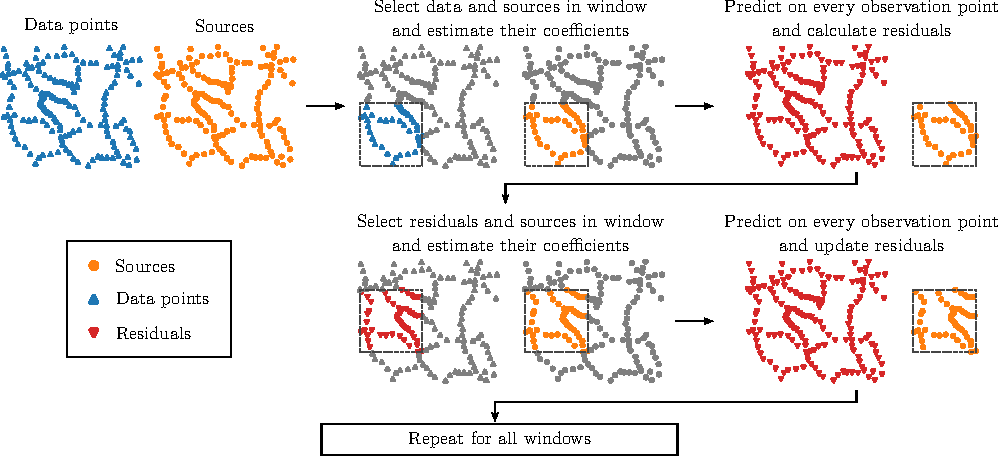
\includegraphics[width=\linewidth]{figs/eql-gradient-boosted/gradient-boosting-schematics.pdf}
    \caption{
        Bosquejo del algoritmo de fuentes equivalentes potenciadas por el
        gradiente.
        Los puntos de datos están representados por triángulos azules
        (orientados hacia arriba), las fuentes equivalentes por puntos naranja,
        los residuos por triángulos rojos (orientados hacia abajo), y los
        límites de la ventana actual por líneas negras de a trazos.
        El algoritmo comienza seleccionado los datos y las fuentes que caen
        dentro de la primer ventana y continua estimando los coeficientes de
        estas fuentes utilizando los puntos de datos seleccionados.
        Luego, se calcula el efecto de las fuentes ajustadas sobre todos los
        puntos de observación y usamos los datos para calcular los residuos.
        Se utiliza otra ventana para seleccionar otro conjunto de residuos
        y fuentes, se estiman sus coeficientes utilizando los residuos
        seleccionados en vez de los datos originales.
        Nuevamente, el efecto de las fuentes estimadas es calculado sobre todos
        los puntos de observación y se actualizan los residuos.
        Estos pasos son repetidos para cada ventana en orden aleatorio.
    }
    \label{fig:gradient-boosting-schematics}
\end{figure}

Vale la pena notar que los dos conjuntos de fuentes equivalentes
correspondientes a dos ventanas solapadas contiguas poseen una porción de sus
fuentes las mismas ubicaciones, específicamente aquellas que caen en la
intersección de ambas ventanas.
Esto nos permite interpretar que el algoritmo de potenciación de gradiente
ajusta los coeficientes de las fuentes múltiples veces: una vez por cada
ventana que cubre cada una de las fuentes.
Este hecho puede ser explotado con el objetivo de ahorrar memoria.
En vez de almacenar todos los vectores $\mathbf{c}_k$
(ec.~\ref{eq:gb-linear-model}), podemos inicializar un único vector
$\mathbf{c}$ con ceros, donde cada elemento representa el coeficiente de cada
una de las $M$ fuentes originales.
Luego de cada iteración del algoritmo de potenciación por gradiente, añadimos
los coeficientes estimados $\hat{\mathbf{c}}_k$ a sus correspondientes
elementos del vector
$\mathbf{c}$.
Dado que la función de modelado directo es lineal, podemos calcular el campo
resultante mediante la ec.~\ref{eq:eql-forward} en vez de utiliza la
ec.~\ref{eq:eql-forward-gb}.
De esta forma, la cantidad de memoria necesaria para almacenar el conjunto
completo de coeficientes se limita a un único vector de $M$ elementos.

Nuestro algoritmo de potenciado por el gradiente es similar a la \emph{boostrap
inversion} utilizada por \citet{vonfrese1988}, la cual también ajusta
iterativamente porciones del modelo de fuentes equivalentes a datos residuales.
Las diferencias claves entre este y nuestro método son:
(i)~las fuentes en las porciones de solapamiento de las ventanas son ajustadas
más de una vez, permitiendo al algoritmo autocorregirse en caso de soluciones
de baja calidad sobre alguna de las ventanas;
(ii)~utilizamos solo los datos dentro de las ventanas durante el ajuste, lo
cual permite la aplicación del algoritmo a conjuntos de datos más grandes.


\subsection{Ubicación de las fuentes}
\label{sec:source_distribution}

La cantidad ideal de fuentes y sus ubicaciones, tanto horizontales como
verticales, han sido debatidas desde la concepción de la técnica de fuentes
equivalentes de la mano de \citet{dampney1969}.
Las elecciones que se realizan con respecto a estos parámetros juegan un rol
importante en la precisión de las predicciones y de los recursos
computacionales necesarios para estimar los coeficientes de las fuentes.
Una distribución ideal de fuentes debería ser simultáneamente capaz de
reproducir los datos observados en los puntos de muestreo, realizar
predicciones precisas en locaciones no muestreadas y minimizar el costo
computacional necesario.

Un gran número de fuentes homogéneamente distribuidas a lo largo y ancho de la
zona de estudio son capaces de reproducir los datos observados.
Sin embargo, los costos computacionales pueden ser prohibitivos y los problemas
subdeterminados que generan son susceptibles a sobreajustar a los datos,
resultando en interpolaciones y extrapolaciones de baja calidad.
En el otro extremo, la utilización de pocas fuentes reduciría el costo
computacional, pero el modelo podría ser incapaz de reproducir el espectro
completo de los datos observados.

Las características particulares de cada muestra juegan también un rol
importante en la elección de la distribución de las fuentes equivalentes.
En el caso de muestras tomadas sobre la superficie terrestre, las observaciones
suelen localizarse a lo largo de trayectorias irregulares junto con algunos
puntos dispersos.
La cobertura de la región de muestreo es usualmente despareja, dejando grandes
áreas sin ninguna medición.
Por otro lado, las observaciones realizadas mediante vehículos aéreos suelen
estar localizadas a lo largo de líneas de vuelo casi rectas y con poca
separación.
Las mediciones se suelen tomar a intervalos muy cortos, produciendo una gran
densidad de datos a lo largo de las líneas de vuelo.
Esto genera un sesgo en el muestreo, lo cual puede producir artefactos de
\emph{aliasing} en las grillas posteriores.

\subsubsection{Distribuciones horizontales de las fuentes}

\begin{figure}[tb]
    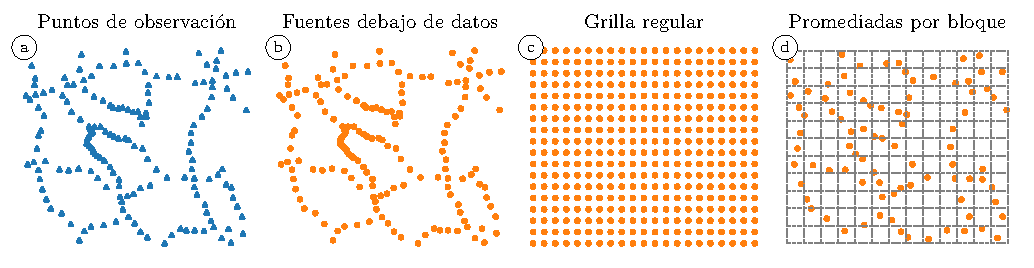
\includegraphics[width=\linewidth]{figs/eql-gradient-boosted/source-layouts-schematics.pdf}
    \caption{
        Bosquejo de las diferentes distribuciones horizontales para los modelos
        de fuentes equivalentes.
        Los puntos azules representan las ubicaciones de las observaciones,
        y los puntos naranja, las ubicaciones de las fuentes equivalentes según
        las distintas estrategias de distribución.
        (a)~Conjunto de \SourceLayoutsSchematicsObservations{} puntos de
        observación que emulan una muestra terrestre.
        (b)~Ubicación de \SourceLayoutsSchematicsSourceBelowData{} fuentes
        obtenidas mediante la distribución \emph{fuentes debajo de datos}.
        (c)~Ubicación de \SourceLayoutsSchematicsGridSources{} fuentes
        obtenidas mediante la distribución \emph{grilla regular}.
        (d)~Ubicación de \SourceLayoutsSchematicsBlockAveragedSources{} fuentes
        obtenidas mediante la distribución \emph{fuentes promediadas por bloque}.
        Las líneas de a trazos grises representan los bloques espaciales dentro
        de los cuales la localización media de los datos es calculada.
    }
    \label{fig:source_layouts}
\end{figure}

Las distribuciones más utilizadas para localizar las fuentes equivalentes
horizontalmente son:

\begin{enumerate}
  \item
    \emph{Fuentes debajo de datos}: una única fuente equivalente es ubicada en
    la misma localización horizontal de cada dato
    (Fig.~\ref{fig:source_layouts}b), pero a diferente altitud. Por lo tanto,
    la cantidad de fuentes es igual a la cantidad de observaciones ($M=N$).
  \item
    \emph{Grilla regular}: una distribución homogénea de fuentes debajo de la
    zona de estudio (Fig.~\ref{fig:source_layouts}c). En la práctica, esto
    suele generar problemas subdeterminados, ya que se requieren mayores
    cantidades de fuentes que de datos ($M>N$).
\end{enumerate}

En el caso de muestras terrestres, la distribución de \emph{grilla regular}
necesita un espaciado entre los nodos lo suficientemente pequeño para poder ser
capaz de ajustar a los datos observados.
Esto genera una cantidad de fuentes innecesariamente grande en regiones donde
no se han realizado observaciones.
En contraste, la distribución \emph{fuentes debajo de datos} es más propensa
a ajustar de manera precisa a los datos observados haciendo uso de una cantidad
menor de fuentes, y por ende reduciendo el costo computacional.
Sin embargo, cuando esta distribución es aplicada a muestras aéreas, la
distribución \emph{fuentes debajo de datos} ubicará una cantidad
indeseablemente grande de fuentes debajo de las líneas de vuelo.
Esto puede conllevar la generación de efectos de \emph{aliasing} sobre los
valores predichos, como un patrón de rayas paralelas a las líneas de vuelo que
suelen observarse en grillas obtenidas de vuelos aeromagnéticos.
La distribución de \emph{grilla regular} puede evitar estos efectos al
distribuir homogéneamente las fuentes y utilizando una capa de fuentes de
densidades continuas (por ejemplo, prismas rectangulares o tesseroides).

Aquí proponemos un nuevo tipo de distribución horizontal de fuentes
equivalentes que puede simultáneamente reducir el costo computacional y mitigar
algunas de las desventajas de las distribuciones existentes.
En la distribución de \emph{fuentes promediadas por bloque}
(\emph{block-averaging sources} en inglés), cada fuente es ubicada en la
posición media de los puntos de datos que caen dentro de un determinado bloque
espacial (Fig.~\ref{fig:source_layouts}d).
Esto se realiza de la siguiente forma:

\begin{enumerate}
    \item Dividir la región de estudio en bloques rectangulares de mismo
        tamaño.
    \item \label{item:median-position} Calcular la media de las posiciones
        horizontales de los puntos de observación que caen dentro de cada
        bloque. Los bloques sin ningún punto de observación son omitidos.
    \item Asignar una fuente puntual a cada posición horizontal media calculada
        en el paso \ref{item:median-position}.
\end{enumerate}

La cantidad total de fuentes creadas por esta nueva distribución será menor que
el número total de observaciones si el tamaño de los bloques es elegido
apropiadamente (asegurándose de que los bloques sean lo suficientemente grandes
como para contener más de un único punto de observación).
El problema sobredeterminado que surge de esta distribución posee un costo
computacional inferior y es menos propenso a sobreajustar los datos, ya que la
complejidad del modelo es menor.
Además, el proceso de \emph{promediado por bloques} puede balancear el
espaciado entre fuentes a lo largo de líneas de vuelo y entre líneas contiguas,
ayudando a reducir los efectos de \emph{aliasing} en las grillas que se generan.
En la sección~\ref{sec:synthetic_distributions}, demostramos mediante pruebas
sobre datos sintéticos que las \emph{fuentes promediadas por bloque} son
capaces de realizar interpolaciones con una precisión comparable a la obtenida
por las otras dos distribuciones, pero utilizando una fracción de fuentes
equivalentes.


\subsubsection{Profundidad de las fuentes}

\begin{figure}[tb]
    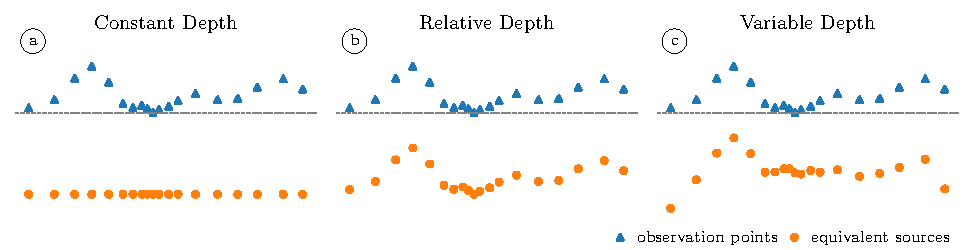
\includegraphics[width=\linewidth]{figs/eql-gradient-boosted/depth_types.pdf}
    \caption{
        Ejemplos de diferentes estrategias para asignar profundidades a las
        fuentes equivalentes.
        Asignaremos una única fuente por cada punto de observación,
        localizándolas en la mismas coordenadas horizontales que los puntos de
        datos.
        Las profundidades de las fuentes son
        (a)~una \emph{profundidad constante} a una determinada coordenada
        vertical,
        (b)~una \emph{profundidad relativa} determinada al desplazar
        uniformemente la coordenada vertical de los puntos de datos hacia
        abajo, y
        (c)~una \emph{profundidad variable} determinada por el desplazamiento
        de la coordenada vertical de los puntos de observación por una cantidad
        proporcional a la distancia media entre fuentes vecinas.
        La distancia entre puntos de datos y sus respectivas fuentes (a)
        depende de la altitud de las observaciones, (b) es constante, y (c) es
        proporcional a la distancia horizontal de las fuentes.
        Vale notar cómo las fuentes agrupadas en el centro del perfil (c) se
        encuentran más someras que sus contrapartes en (b).
    }
    \label{fig:depth_types}
\end{figure}

Es ampliamente conocido de la teoría de potencial que la profundidad de una
fuente puntual influencia la longitud de onda del campo observado en la
superficie.
Esto hace que la profundidad de la fuente sea un parámetro clave que afecta el
producto de la interpolación y otras operaciones realizadas mediante fuentes
equivalentes.
En la literatura podemos encontrar múltiples estrategias diferentes para
asignar profundidad de las fuentes.
Aquí destacaremos las siguientes (Fig.~\ref{fig:depth_types}):

\begin{enumerate}
  \item
    \emph{Profundidad constante}:
    La opción más simple es ubicar todas las fuentes a la misma profundidad
    (Fig.~\ref{fig:depth_types}a).
    Si las mediciones fueron obtenidas a altitudes significativamente diversas,
    algunas mediciones se encontrarán más distantes a las fuentes que otras,
    lo que podría generar problemas a la hora de reproducir las longitudes de
    onda más cortas en los puntos de grandes altitudes.
 \item
    \emph{Profundidad relativa}:
    Las profundidades de las fuentes se determinan al desplazar la coordenada
    vertical de los puntos de datos hacia abajo por una cantidad constante
    (Fig.~\ref{fig:depth_types}b).
    Las fuentes no tendrán todas las mismas coordenadas verticales, pero se
    encontrarán todas a la misma distancia vertical con respecto a los puntos
    de observación.
 \item
    \emph{Profundidad variable}:
    Las profundidades de las fuentes son proporcionales a la distancia
    horizontal entre primeros vecinos de datos o fuentes (Fig.~\ref{fig:depth_types}c).
    Diferentes variaciones de esta estrategia han sido propuestas
    anteriormente, por ejemplo
    \citet{cordell1992}, \citet{guspi2004}, y \citet{guspi2009}.
    La razón fundamental para utilizar esta estrategia surge en caso de que la
    muestra posea puntos muy agrupados (formando \emph{clusters} o cúmulos) en
    algunas áreas, es posible que deseemos ubicar las fuentes debajo de ellas
    a menores profundidades, con el objetivo de preservar las longitudes de
    onda más cortas presentes en esos datos.
\end{enumerate}

Nuestro enfoque sobre la estrategia de \emph{profundidad variable} será:

\begin{equation}
  z = z_{obs} + \Delta z + \alpha h,
  \label{eq:variable_depth}
\end{equation}

\noindent
donde $z$ es la coordenada vertical (positiva hacia abajo) de una fuente
equivalente,
$\Delta z$ es un desplazamiento relativo en profundidad que se aplica de manera
uniforme a todas las fuentes,
$\alpha$ es un \emph{factor de profundidad} adimensional,
$h$ es la distancia horizontal media a las primeras $k$ fuentes vecinas,
y
$z_{obs}$ es una coordenada vertical relacionada a los puntos de observación
que dependerá de la estrategia horizontal utilizada.
Para \emph{fuentes debajo de datos}, será la coordenada vertical del
punto de observación correspondiente a la fuente.
Para una \emph{grilla regular}, puede ser interpolada a partir de la coordenada
vertical de todos los puntos de datos.
Finalmente, para \emph{fuentes promediadas por bloque} será la coordenada
vertical media de todos los puntos de datos que caen dentro del bloque
correspondiente a la fuente.

En la sección~\ref{sec:synthetic_distributions}, probamos la efectividad de
estas estrategias sobre datos sintéticos.

%%%%%%%%%%%%%%%%%%%%%%%%%%%%%%%%%%%%%%%%%%%%%%%%%%%%%%%%%%%%%%%%%%%%%%%%%%%%%%%

\section{Tests on synthetic data}

\begin{figure*}[tb]
    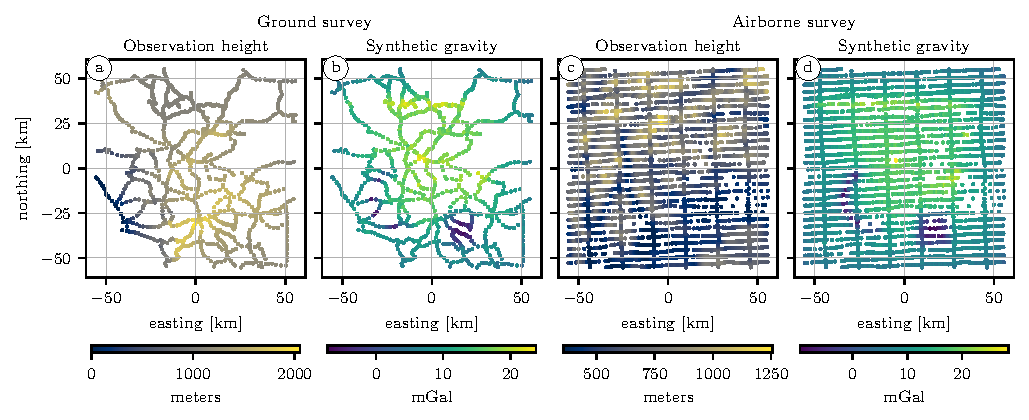
\includegraphics[width=\linewidth]{figs/eql-gradient-boosted/synthetic-survey-layouts.pdf}
    \caption{
        Observation heights and gravity values for the synthetic ground (a-b)
        and airborne (c-d) surveys.
        Heights are given in meters above the zero height plane.
        The synthetic gravity data are contaminated with pseudo-random Gaussian
        noise with zero mean and \SurveyNoise{} standard deviation.
    }
    \label{fig:synthetic-layouts}
\end{figure*}

\begin{figure}[tb]
    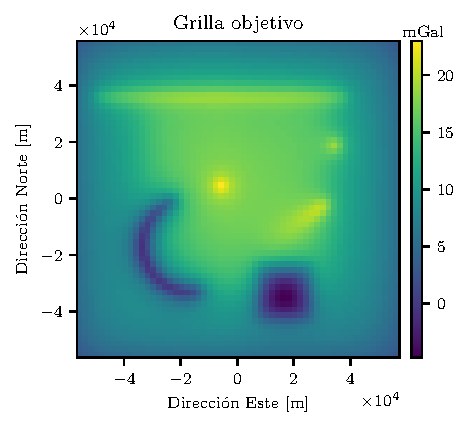
\includegraphics[width=\linewidth]{figs/eql-gradient-boosted/target-grid.pdf}
    \caption{
        Pseudo-color map of the target grid of synthetic gravity data. The grid
        is composed of \TargetEastingSize{}$\times$\TargetNorthingSize{} points
        with a spacing of \TargetSpacing{}. The grid height is \TargetHeight{}
        above the zero height plane.
    }
    \label{fig:synthetic-target}
\end{figure}

We have used synthetic gravity datasets to test the interpolation accuracy of
the difference horizontal and vertical source distribution strategies as well
as the gradient-boosted equivalent sources method.
To generate the data, we created a model of \NPrisms{} right-rectangular
prisms,
distributed in a \ModelEasting{}$\times$\ModelNorthing{} area with depths
varying between \ModelDepth{} and zero.
The density contrast of prisms ranges from \ModelMinDensity{} to
\ModelMaxDensity{}.
The model includes prisms of different shapes, sizes, and depths to create
gravity disturbances with a variety of wavelengths.

We created two synthetic datasets from the model, one simulating a ground
survey and another an airborne acquisition (Fig.~\ref{fig:synthetic-layouts}).
To create the synthetic ground survey, we selected measurement positions from a
portion of a public domain gravity dataset for Southern Africa, available
through the NOAA National Centers for Environmental Information (NCEI).
For the synthetic airborne survey, we used a portion of the Great Britain
Aeromagnetic Survey acquired by Hunting Geology and Geophysics Ltd and Canadian
Aeroservices Ltd between 1955 and 1965 and made publicly available by the
British Geological Survey (BGS).
In both cases, we rescaled the horizontal coordinates of each survey portion to
span an area of \SurveyEasting{}$\times$\SurveyNorthing{}, matching the model
dimensions.
The ground survey contains \GroundSurveyPoints{} observations distributed at
heights between \GroundSurveyMinHeight{} and \GroundSurveyMaxHeight{}
(Fig.~\ref{fig:synthetic-layouts}a).
The airborne survey has \AirborneSurveyPoints{} observations at heights between
\AirborneSurveyMinHeight{} and \AirborneSurveyMaxHeight{}
(Fig.~\ref{fig:synthetic-layouts}c).

The vertical component of the gravitational acceleration generated by the
model was computed  using the method of \citet{nagy2000, nagy2002}
with recent modifications by \citet{fukushima2020},
as implemented in the open-source software Harmonica \citep{harmonica2021}.
We generated a \emph{target grid} of
\TargetEastingSize{}$\times$\TargetNorthingSize{} points with a spacing of
\TargetSpacing{} and located \TargetHeight{} above the zero height plane
(Fig.~\ref{fig:synthetic-target}) to serve as a reference when calculating the
interpolation error.
We then generated synthetic ground (Fig.~\ref{fig:synthetic-layouts}b) and
airborne (Fig.~\ref{fig:synthetic-layouts}d) data to which we added
pseudo-random Gaussian noise with zero mean and \SurveyNoise{} standard
deviation.


\subsection{Source distribution strategies}
\label{sec:synthetic_distributions}

\begin{figure*}[p]
    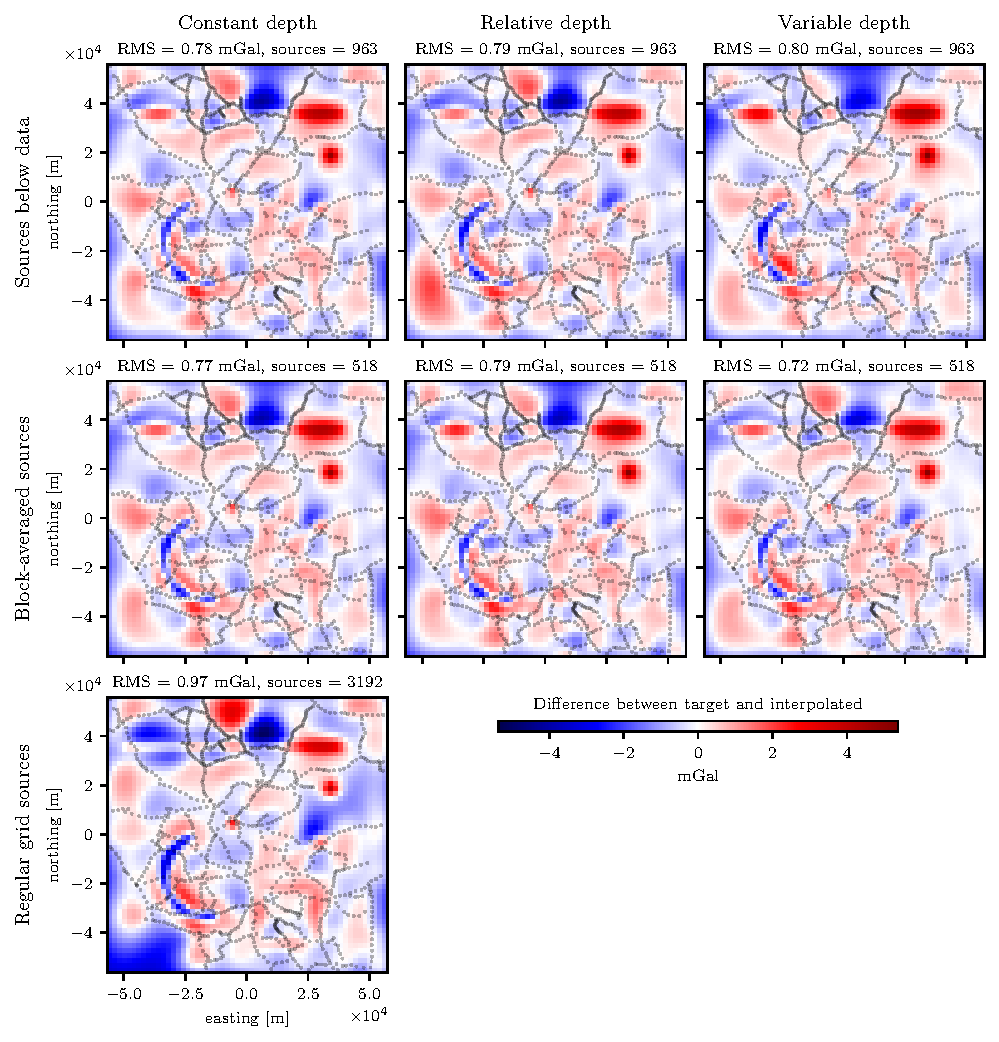
\includegraphics[width=\linewidth]{figs/eql-gradient-boosted/ground_survey_differences.pdf}
    \caption{
        Pseudo-color maps of the differences between the target grid and the
        interpolated synthetic ground survey data produced by each source
        distribution strategy.
        The black dots represent the horizontal location of the synthetic data
        points. The RMS error and total number of equivalent sources is
        reported for each strategy at the top of the respective maps.
    }
    \label{fig:ground-survey-differences}
\end{figure*}

\begin{figure*}[p]
    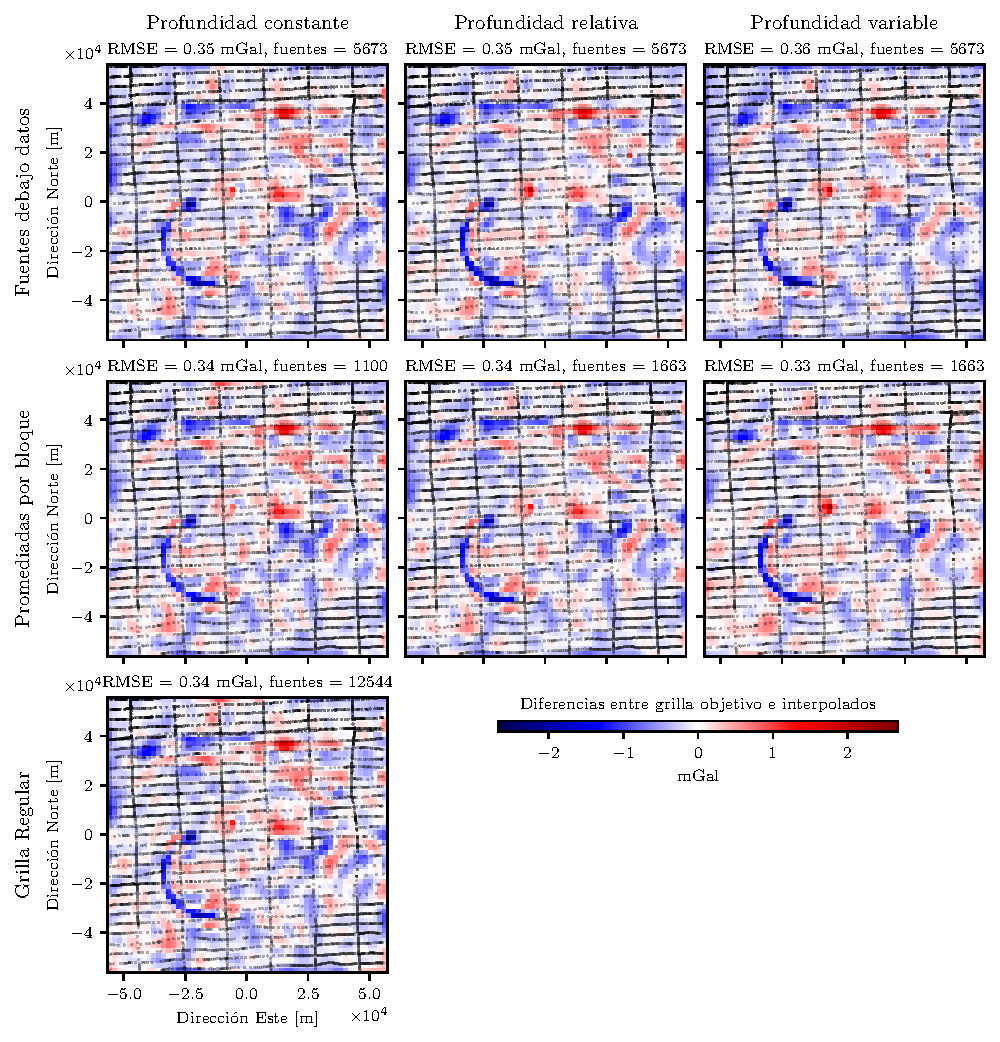
\includegraphics[width=\linewidth]{figs/eql-gradient-boosted/airborne_survey_differences.pdf}
    \caption{
        Pseudo-color maps of the differences between the target grid and the
        interpolated synthetic airborne survey data produced by each source
        distribution strategy.
        The black dots represent the horizontal location of the synthetic data
        points. The RMS error and total number of equivalent sources is
        reported for each strategy at the top of the respective maps.
    }
    \label{fig:airborne-survey-differences}
\end{figure*}

We investigated the effect on interpolation accuracy of different strategies
for distributing the equivalent sources horizontally and vertically.
To do this, we used the damped least-squares solution described in
Section~\ref{sec:eql_inversion} (without gradient boosting) to interpolate the
synthetic datasets (Fig.~\ref{fig:synthetic-layouts}) and compared the results
against the target grid (Fig.~\ref{fig:synthetic-target}).
This process was repeated for each combination of horizontal layout
(\emph{sources below data} and \emph{block-averaged sources}) and depth type
(\emph{constant}, \emph{relative}, and \emph{variable}) and for regular grid
sources with a constant depth, totalling 7 different combinations.

Each source distribution strategy requires certain hyper-parameters to be
chosen in order to build the set of point sources.
For example, using a constant depth needs the definition of the depth and using
block-averaged sources requires the definition of the block size.
The predictive capabilities of the equivalent sources depend on the choice of
these hyper-parameters.
To ensure that our comparisons are fair, we perform an exhaustive search over
combinations of hyper-parameter values (including the damping parameter from
Eq.~\ref{eq:misfit}) to obtain the best prediction that can be achieved by each
source distribution strategy.
Here, the best prediction is defined as the one that minimizes the root
mean-square error (RMS) between interpolated values and the target grid
(Fig.~\ref{fig:synthetic-target}).
The parameter values used in these searches and the one producing the smallest
RMS error are outlined in Tables~\ref{tab:parameters-ground-survey}
and~\ref{tab:parameters-airborne-survey}.

Fig.~\ref{fig:ground-survey-differences}
and~\ref{fig:airborne-survey-differences} show the differences between the
target grid and the best prediction achieved by each source distribution
strategy for the ground and airborne synthetic surveys, respectively.
For the synthetic ground survey, the horizontal layouts produced similar RMS
values of approximately 0.8\mGal{} regardless of the depth type, with the
exception of the regular grid layout which produced a larger RMS of
\BestGroundGridSourcesConstantDepthRms{}\mGal{}.
The differences between the target grid and the interpolated values are larger
in regions of poor data coverage.
Edge effects are present for all strategies but are noticeably smaller for the
combination of block-averaged sources with a variable depth based on the
nearest neighbour distance.
For the synthetic airborne survey, all strategies (including the regular grid)
produced similar RMS errors of approximately 0.3\mGal{}.
The maps of the differences between the target grid and interpolation results
are visually indistinguishable from each other.

%%%%%%%%%%%%%%%%%%%%%%%%%%%%%%%%%%%%%%%%%%%%%%%%%%%%%%%%%%%%%%%%%%%%%%%%%%%%%%%


\subsection{Window size and overlap in gradient boosting}
\label{sec:window_size_and_overlap}

We assessed the trade-offs in interpolation accuracy and computation time of
the gradient-boosted equivalent sources algorithm as a function of the two key
controlling factors: the window size and the amount of overlap between adjacent
windows.
The comparisons were performed against a regular least-squares solution
(Eq.~\ref{eq:least_squares_solution}) using the synthetic airborne data
(Fig.~\ref{fig:synthetic-layouts}c-d).
To avoid biasing the results, we used the same locations of equivalent sources
for both the regular and gradient-boosted interpolations, namely
block-averaged sources with a block size of
\BestAirborneBlockAveragedSourcesRelativeDepthSpacing\m{} and a
relative depth of
\BestAirborneBlockAveragedSourcesRelativeDepthDepth\m{}.

\subsubsection{Window size}
\label{sec:window_size}

The size of the windows controls the size of the Jacobian matrices
$\tilde{\mathbf{A}}_k$ by limiting the number of data points and equivalent
sources used in each step of the gradient-boosting algorithm
(Alg.~\ref{alg:gradient_boosting_window}).
Thus, using smaller windows will reduce the total amount of computer memory
required to estimate the source coefficients.
Nevertheless, smaller windows may produce less accurate interpolations by
failing to achieve the global minimum of the goal function in
Eq.~\ref{eq:misfit}.
The window size might also impact the computation time in non-intuitive ways
since smaller windows generate smaller least-squares problems but also require
more gradient-boosting iterations.

We calculated the interpolation RMS error (between the interpolated grid and
the target grid in Fig.~\ref{fig:synthetic-target}) and computation time for a
fixed window overlap of 50\% and several window sizes.
To avoid any biases introduced by the shuffling of windows, the calculations
were repeated using different seeds for the pseudo-random number generator used
in the shuffling.
Fig.~\ref{fig:gradient-boosted-comparison}a shows the RMS error and
Fig.~\ref{fig:gradient-boosted-comparison}c shows the computation time
required for estimating the source coefficients, both as functions of
the window size.

\begin{figure*}[tb]
    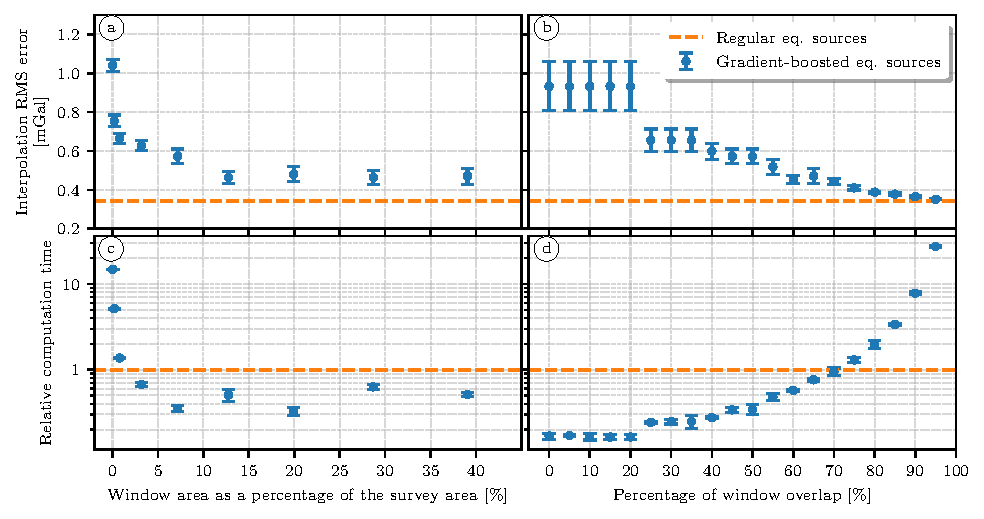
\includegraphics[width=\linewidth]{figs/eql-gradient-boosted/gradient-boosted-comparisons.pdf}
    \caption{
        Interpolation RMS error (a-b) and relative computation time (c-d) for
        regular least-squares equivalent sources (orange dashed lines) and
        gradient-boosted equivalent sources (blue dots and error bars).
        Window overlap is given as a percentage of the window size (an overlap
        of 50\% means that two adjacent windows share an area half of the size
        of the entire window).
        For gradient-boosting, the RMS errors and computation times are the
        means (error bars are 1 standard deviation) of results using different
        seeds for the pseudo-random number generator.
        Computation time is the ratio between the time required to estimate the
        source coefficients for the gradient-boosted and the regular equivalent
        sources.
}
    \label{fig:gradient-boosted-comparison}
\end{figure*}

These results show that the interpolation error for gradient-boosting is
generally larger than the error for regular equivalent sources.
The error decreases asymptotically to within $\sim 40\%$ of the regular
equivalent sources for windows with an area greater than $\sim 10\%$ of the
survey area.
The computation time similarly decreases with window size, with the
gradient-boosting being generally faster than the regular equivalent sources
for windows with an area greater than $\sim 5\%$ of the survey area.
As the window size increases, both RMS error and computation time appear to
stabilize to nearly constant levels.

\subsubsection{Window overlap}

The amount of overlap between adjacent windows plays an important role in the
performance of the gradient-boosted equivalent sources.
It controls the number of iterations and how many times a particular source is
used in the least-squares fitting process.
The experiments in the previous section showed that 50\% overlap was
sufficient to achieve acceptable interpolation accuracy.
However, we studied separately the impacts of the amount of window overlap on
both accuracy and computation time.

We performed a similar experiment to the one in section~\ref{sec:window_size}
but this time kept the window size fixed to \BoostOverlappingWindowSize{} and
varied the amount of overlap from 0\% to 95\% with a step size of 5\%.
All other experimental procedures remained unchanged.
Fig.~\ref{fig:gradient-boosted-comparison}b shows the RMS error and
Fig.~\ref{fig:gradient-boosted-comparison}d shows the computation time
required for estimating the source coefficients, both as functions of
the window overlap.

Our results show that the interpolation RMS error decreases with the amount of
overlap, reaching the same accuracy as the regular equivalent sources at
approximately 90\% overlap.
On the other hand, the computation time increases with the amount of overlap,
becoming larger than that of the regular equivalent sources for overlaps
greater than 70\%.
This is expected since increasing the overlap adds iterations to the gradient
boosting algorithm without decreasing the individual least-squares problem
sizes to compensate.


\subsection{
    Interpolation with gradient boosting
}
\label{sec:gb_interpolation}

Finally, we applied the gradient-boosted equivalent sources to interpolate the
synthetic airborne survey (Fig.~\ref{fig:synthetic-layouts}).
As previously, we used the block-averaged sources layout with a block size of
\EqlBoostAirborneSpacing{}.
Based on the results from section \ref{sec:window_size_and_overlap}, we adopted
a window overlap of 50\% and a window size of \EqlBoostAirborneWindowSize{}.

We estimated the relative depth of the sources and the damping parameter by
comparing the predictions against the values of the target grid.
The search explored \emph{depth} values between \EqlBoostAirborneMinDepth{} and
\EqlBoostAirborneMaxDepth{} and \emph{damping} values between
\EqlBoostAirborneMinDamping{} and \EqlBoostAirborneMaxDamping{} by steps of one
order of magnitude.
The most accurate predictions achieved a RMS error of
\EqlBoostAirborneRmsScore{} with a depth of \EqlBoostAirborneDepth{} and
a damping of \EqlBoostAirborneDamping{}.
It is worth noting that the RMS error achieved by the gradient-boosted
equivalent sources is comparable to the ones obtained by the regular equivalent
sources in Section \ref{sec:synthetic_distributions}.
To highlight the importance of randomizing the order of windows in the
gradient-boosting iterations, we preformed the interpolation once more using
the same values of \emph{damping} and \emph{depth} but this time iterating over
windows in sequential order (South to North, West to East).

\begin{figure}[tb]
    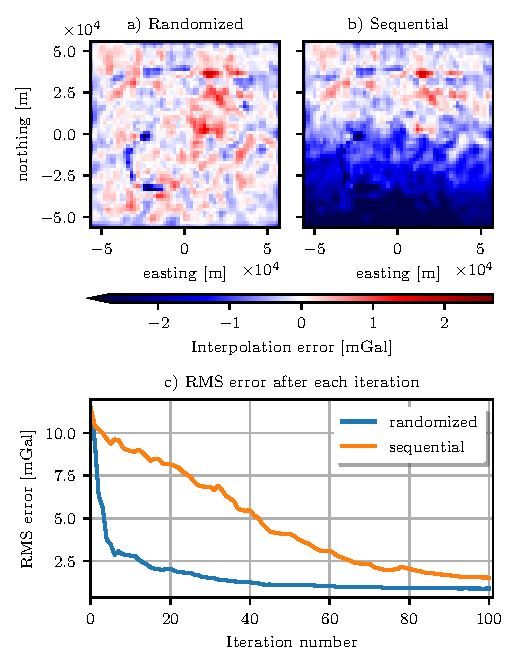
\includegraphics[width=\linewidth]{figs/eql-gradient-boosted/eql-boost-airborne.pdf}
    \caption{
        Interpolation error for gradient-boosted equivalent sources using
        randomized (a) and sequential (b) window order.
        (a and b)~Pseudo-color maps of the differences between the target grid
        and the interpolated synthetic airborne survey data.
        The color scale has been cropped to the same range as
        Fig.~\ref{fig:airborne-survey-differences}.
        (c)~Root-mean squared error after each iteration of the
        gradient-boosting algorithm.
}
\label{fig:eql-boost-airborne}
\end{figure}

Figs.~\ref{fig:eql-boost-airborne}a-b show the differences between the target
grid and the interpolation results for windows in randomized and sequential
order, respectively.
The differences for randomized windows resemble those for regular least-squares
equivalent sources seen in Figs.~\ref{fig:ground-survey-differences} and
\ref{fig:airborne-survey-differences}.
On the other hand, the differences for sequential windows show a clear
trend of large negative differences in the South decreasing towards the North.
This trend is correlated with the order in which windows are executed, with
differences decreasing in absolute value towards the end of the algorithm.
Fig.~\ref{fig:eql-boost-airborne}c shows the RMS error of the fitting process
after each iteration for both window orders, clearly indicating that
a randomized window order leads to faster convergence of the algorithm.


%%%%%%%%%%%%%%%%%%%%%%%%%%%%%%%%%%%%%%%%%%%%%%%%%%%%%%%%%%%%%%%%%%%%%%%%%%%%%%%

\section{Gridding gravity data from Australia}

\begin{figure*}[p]
    \includegraphics[width=\linewidth]{figs/eql-gradient-boosted/australia.png}
    \caption{
      Pseudo-color maps of observed (a and c) and
      interpolated (b and d) gravity disturbance of Australia.
      The observed values in a and c are plotted as colored circles.
      The red rectangle marks the boundaries of the highlight maps in c
      and d.
      Observations are part of a compilation by \citet{wynne2018} of
      over 1.7 million ground gravity measurements.
      Interpolated values were obtained through gradient-boosted equivalent
      sources and calculated on a regular grid at \AustraliaEqlGridHeight{}
      over the WGS84 ellipsoid.
    }
    \label{fig:australia}
\end{figure*}

This section will demonstrate how gradient-boosted equivalent sources can be
used to interpolate large datasets onto regular grids at uniform height.
For this purpose, we selected an open-access compilation of ground gravity
surveys over Australia made by \citet{wynne2018} and filtered and referenced to
the WGS84 ellipsoid by \citet{australia_compilation}.
It contains over 1.7 million data points and covers most of the Australian
territory at variable point spacings.
Our goal is to create a 1~arc-minute resolution grid of gravity disturbances at
a constant geometric height of \AustraliaEqlGridHeight{} (the largest height of
observations).

We computed the gravity disturbance by removing the normal gravity of
the WGS84 ellipsoid from the observed gravity data (Fig.~\ref{fig:australia}).
Here, normal gravity was computed at each observation point through the
closed-form formula of \citet{ligotze2001} using the Boule software
\citep{boule2020}.
Finally, we converted the observations to planar Cartesian coordinates by
applying a Mercator projection.

We start the interpolation process by defining a set of block-averaged sources
using a block size of 1.8\km{}, resulting in a total of
\AustraliaEqlNSources{}~point sources.
The block size was chosen to match the desired resolution of the final grid
(1~arc-minute is approximately 1.8\km{} at the equator).
Based on the results obtained in Section~\ref{sec:synthetic_distributions}, we
have chosen to use the \emph{relative depth} strategy.
The window overlap was once again fixed at 50\%.
To determine the size of the windows, we calculated the amount of computer memory
needed to store the largest Jacobian matrix for different values of window size
(Fig.~\ref{fig:australia-memory-cv-error}a).
We have chosen a size of \AustraliaEqlWindowSize{} in order to limit the
amount of memory needed to under 16~Gigabytes.

\begin{figure}[tbh!]
    \makeatletter%
    \if@twocolumn%
        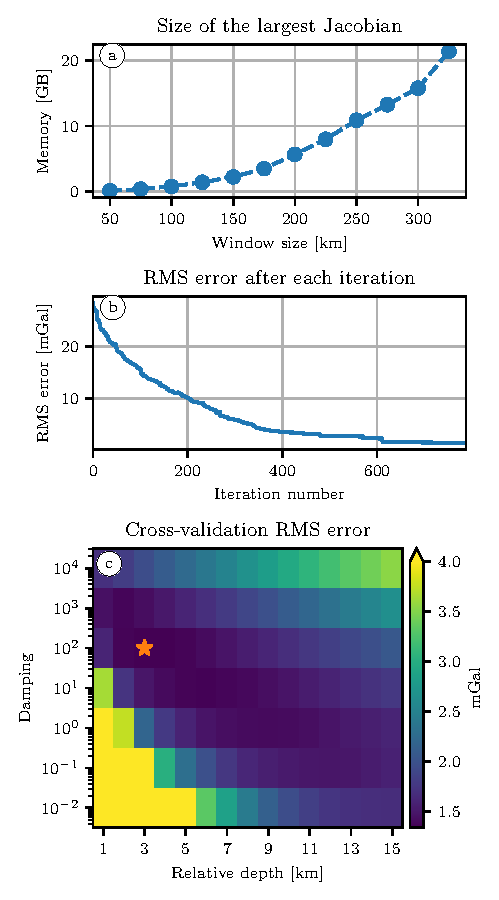
\includegraphics[width=\linewidth]{figs/eql-gradient-boosted/australia-memory-cv-error.pdf}
    \else% \@twocolumnfalse
        \centering
        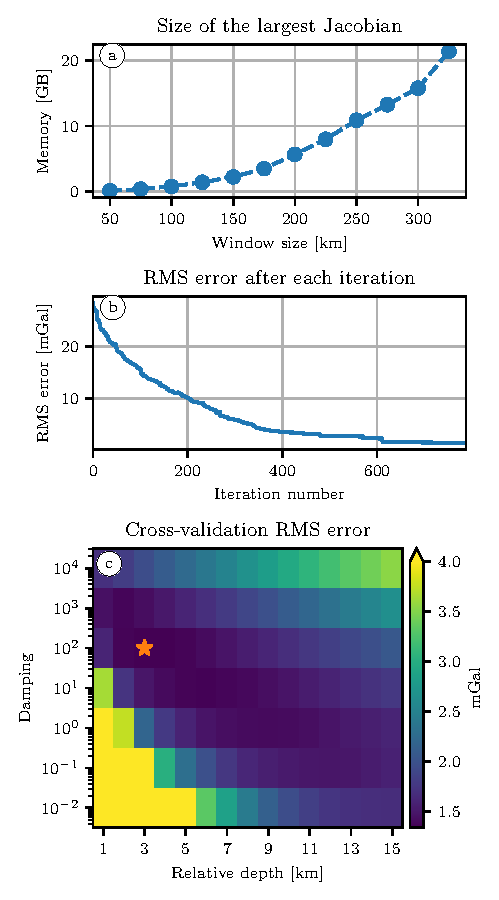
\includegraphics[width=0.6\linewidth]{figs/eql-gradient-boosted/australia-memory-cv-error.pdf}
    \fi
    \makeatother
    \caption{
        (a) Amount of computer memory needed to store the largest Jacobian
        matrix for different window sizes. Our implementation uses double
        precision floating point numbers (64 bits) for the Jacobian.
        (b) Root-mean square error against the observed data after each
        iteration of the gradient-boosting algorithm.
        (c) K-Fold cross-validation root-mean square errors obtained for each
        pair of damping and depth parameters. The orange star highlights the
        minimum.
    }
    \label{fig:australia-memory-cv-error}
\end{figure}

We determined the depth of the sources and the damping parameter by applying
K-Fold cross-validation through the scikit-learn library \citep{sklearn2011}.
The method randomly divides the original data into $k$ sets (folds), fits the
model using only data from $k - 1$ folds, and validates the model by comparing
its predictions against the one remaining fold.
This process is carried out once for each one of the $k$ folds, leading to
an estimated mean cross-validation RMS error for the model.
To speed up the computation, we only performed the cross-validation on a subset
of the data corresponding to an area of
\AustraliaSmallAreaEastingSize{}$\times$\AustraliaSmallAreaNorthingSize{}
containing \AustraliaSmallAreaNPoints{} points.
We ran the cross-validation repeatedly for combinations of \emph{depth},
ranging from \AustraliaDepthMin{} to \AustraliaDepthMax{},
and \emph{damping}, from \AustraliaDampingMin{} to \AustraliaDampingMax{} in
steps of one order of magnitude.
Figure \ref{fig:australia-memory-cv-error}c shows the resulting
cross-validation RMS errors and highlights the minimum value of
\AustraliaEqlRmsScore{}, which corresponds to a relative depth of
\AustraliaEqlDepth{} and a damping equal to \AustraliaEqlDamping{}.

Finally, we proceeded to estimate the source coefficients using the entire
dataset and the parameters previously determined.
The estimated source coefficients were then used to predict the values of the
gravity disturbance on a regular grid of
\AustraliaEqlGridNLongitude{}$\times$\AustraliaEqlGridNLatitude{} points at
\AustraliaEqlGridHeight{} above the ellipsoid.
On a modest workstation with 16 cores and 16~Gigabytes of RAM,
estimating the \AustraliaEqlNSources{} coefficients with gradient-boosting took
$\sim 1.3$~hours and the prediction step took $\sim 18$~minutes.

Fig.~\ref{fig:australia} shows the original data distribution and the
interpolated grid.
Grid points that are further than 50\km{} from the nearest data point are
masked to avoid unrealistic extrapolations.
Fig.~\ref{fig:australia-memory-cv-error}b shows the RMS error against the
observed data after each iteration of the algorithm.
Fig.~\ref{fig:australia-residuals} shows the difference between the observed
and predicted gravity disturbances.
The inset figure shows a histogram of these residuals, which are approximately
normally distributed around zero.

\begin{figure}[tb]
    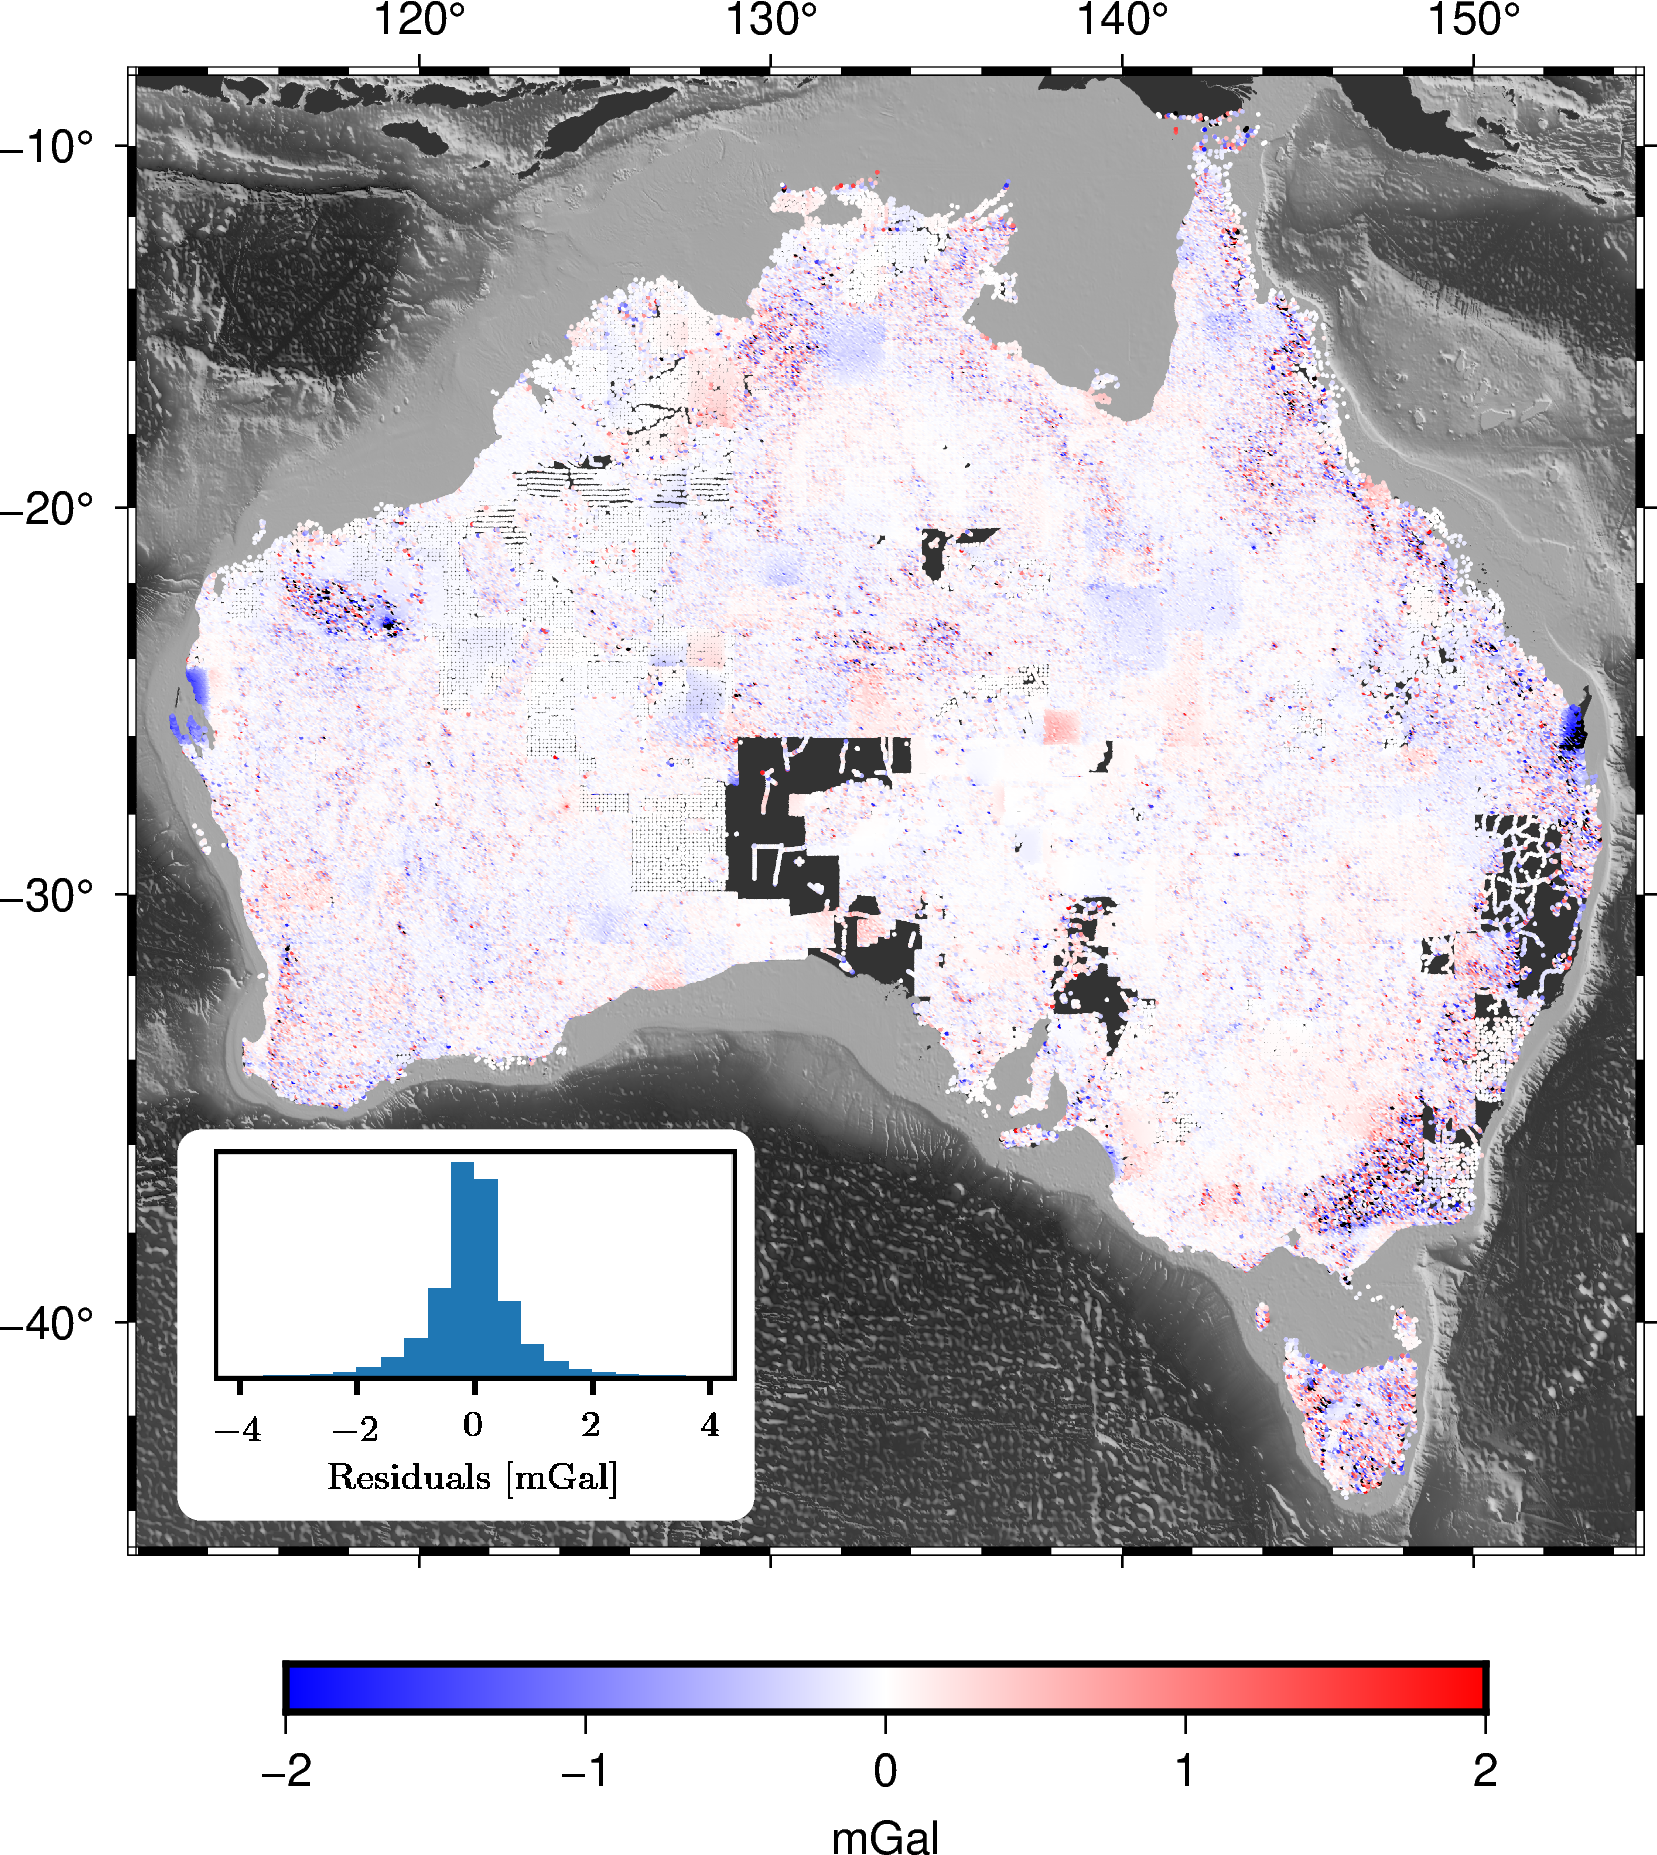
\includegraphics[width=\linewidth]{figs/eql-gradient-boosted/australia-residuals.png}
    \caption{
        Residuals. Differences between the gravity disturbance data from
        Australia and the predicted values by the estimated equivalent sources
        on the same observation points. The color map has been truncated to
        improve the visualization around the largest portion of residual
        values. The inset plot shows a histogram of the residuals.
    }
    \label{fig:australia-residuals}
\end{figure}


%%%%%%%%%%%%%%%%%%%%%%%%%%%%%%%%%%%%%%%%%%%%%%%%%%%%%%%%%%%%%%%%%%%%%%%%%%%%%%%

\section{Discussion}

\subsection{Location of sources}

The results of our tests on synthetic data
(Figs.~\ref{fig:ground-survey-differences}
and~\ref{fig:airborne-survey-differences}) show that there are no significant
differences in interpolation accuracy between source distribution strategies,
both in terms of the interpolation RMS errors and from visual inspection of the
difference maps.
Therefore, we conclude that all source distribution strategies are able to
produce comparable interpolations.
Nevertheless, the \emph{block-averaged sources} strategy makes use of fewer
sources when compared with other strategies, which reduces the computational
load of estimating the sources coefficients and forward modelling.
To ensure that the interpolation is able to reproduce the high frequencies in
the data, the block size used in the averaging should be chosen to match the
desired grid resolution.

The choice of source depth strategy does not appear to significantly impact the
interpolation RMS error.
In the particular case of a sparse ground survey with block-averaged sources,
the use of a variable depth visibly reduced edge effects and artifacts in areas
of poor data coverage.
At a first glance, the choice of a depth strategy would not seem to impact
the computation time.
However, when searching for the set of hyper-parameters that produce the most
accurate interpolation (e.g., through cross-validation), one must solve the
inverse problem once for every possible combination of parameters.
A depth strategy like the \emph{variable depth} requires a higher number of
hyper-parameters (depth shift $\Delta z$, depth factor $\alpha$, and the number
of nearest neighbours $k$ from Eq.~\ref{eq:variable_depth}) than other
strategies which only require a single parameter.
Having more parameters means increasing the dimensions of the parameter space
and thus increasing the number of possible combinations.
Thus, we recommend using a \emph{constant depth} or a \emph{relative depth}
when processing large datasets in order to minimize computation time.

\subsection{Gradient boosting}

From Fig.~\ref{fig:gradient-boosted-comparison}a
and~\ref{fig:gradient-boosted-comparison}c, we can see that the
gradient-boosted equivalent sources produce slightly less accurate
interpolation results but are able to achieve smaller computation times than
regular equivalent sources.
The reduction of the accuracy might be due to the gradient boosting algorithm
failing to converge to the global minimum of the goal function.
As the windows increase in size, interpolation error decreases because more data
points are included into the least-squares fitting of the source coefficients.
At the same time, the fitting process becomes faster because of a reduction in
the number of iterations.
Our results indicate that it is desirable to maximize the window size,
which can be done up to the point that the Jacobian matrices still fit within
the available computer memory.

The results shown in Figs.~\ref{fig:gradient-boosted-comparison}b
and~\ref{fig:gradient-boosted-comparison}d indicate that using
window overlap values between 40\% and 70\% strike a balance between
accuracy and computation time.
This corroborates our initial choice of 50\% overlap, which is good enough for
producing accurate predictions in reasonable times.

Finally, the results in Fig.~\ref{fig:eql-boost-airborne} highlight the
importance of randomizing the order in which the overlapping windows are
iterated.
Running the gradient boosting algorithm sequentially produces less accurate
predictions and decreases the convergence rate of the method.

\subsection{Australia gravity data}

The application of the gradient-boosted equivalent sources to the Australian
gravity dataset demonstrates that the method is able to interpolate and
upward-continue large datasets in a reasonable amount of time using only modest
computational resources.
The resulting grid (Fig.~\ref{fig:australia}) preserves the high resolution of
the original data while avoiding aliasing artifacts due to the block averaging
of the source locations.
Some parts of the grid are smoother and have lower amplitudes than the original
data (e.g., some southwestern parts), which is expected from the upward
continuation that was performed to have the grid at a constant height.
From the cross-validation analysis on a subset of the data, we estimate that
the interpolation error is approximately \AustraliaEqlRmsScore{}.

The largest residuals in Fig.~\ref{fig:australia-residuals} are located in
regions with high-amplitude short-wavelength features in the observed data.
This is expected since the method involves some degree of smoothing because of
the use of damping and the source depths.
There are also low-amplitude long-wavelength residual signals that seem to
coincide with some of the windows of the gradient-boosting method.
A possible cause of these features is inability of the equivalent-sources
within a window to adequately fit the long-wavelength components of the data.
We note, however, that all of these long-wavelength residuals are smaller than
1\mGal{} in amplitude and do not represent a significant source of errors.

The elongated valley around the minimum of the cross-validation RMS errors
(Fig.~\ref{fig:australia-memory-cv-error}c) shows that there is ambiguity in
the choice of damping and source depths.
One could choose a large damping with a small depth or a small damping with a
large depth to achieve roughly the same interpolation result.
This is expected since both parameters control the smoothness of the
interpolation.

%%%%%%%%%%%%%%%%%%%%%%%%%%%%%%%%%%%%%%%%%%%%%%%%%%%%%%%%%%%%%%%%%%%%%%%%%%%%%%%

\section{Conclusions}

The equivalent source technique has been proven to be well suited for
interpolating gravity disturbances and magnetic anomalies.
The two main reasons that make it to stand out from other 2D interpolation
methods is the fact that the equivalent sources take into account the height of
the observations and that the interpolated values will always be harmonic
functions.
The main challenge of using equivalent sources in practice is the high
computational load of estimating the coefficients of the equivalent sources,
specially the computer memory needed to store the Jacobian matrix.

We present two strategies that could be simultaneously applied to interpolate
datasets with millions of points on modest hardware:
block-averaging source locations, which reduces the number of equivalent
sources needed for the interpolation,
and the gradient-boosted equivalent source algorithm, which breaks down the
inverse problem into smaller sets of equivalent sources defined by overlapping
windows.
Both methods were tested against synthetic datasets in order to compare their
accuracy and how they perform in terms of computational efficiency.

Our results show that the block-averaged sources reduce the computational
load needed to estimate source coefficients in comparison to two traditional
strategies (placing sources below data points or on regular grids).
We also show that this reduction of the number of sources does not affect
the accuracy of the predictions.
The use of block-averaged sources may also prevent aliasing of the interpolated
values, specially when the observations are unevenly sampled (e.g., airborne
and shipborne surveys).
Special attention must be payed when choosing the size of the blocks for
averaging.
As a thumb rule, we recommend choosing a size approximately equal to
the resolution of the regular grid where the values will be interpolated.

Tests that compared strategies for the vertical location of the
sources showed that any one of the three strategies tested
(\emph{constant depth}, \emph{relative depth} and \emph{variable depth})
produces comparable accuracy of interpolation.
Nevertheless, we are more prone to recommending either the \emph{constant
depth} or the \emph{relative depth} for most applications because they involve
less hyper-parameters that would need to be configured before the actual
interpolation.

Gradient-boosted equivalent sources were shown to heavily reduce the computer
memory needed to estimate source coefficients, making it possible to
interpolate large datasets with millions of points that would otherwise produce
Jacobian matrices larger than the available memory.
The interpolations obtained though this new method achieve close to the same
accuracy than the regular equivalent sources, while reducing the computation
time by approximately a factor of three.
We also show that an overlap of 50\% between adjacent windows achieves a good
compromise between accuracy and computation time.
The size of the overlapping windows should be chosen as the maximum value
possible that creates Jacobian matrices that still fit into computer memory.
Moreover, randomizing the order in which the windows are iterated increases the
convergence rate of the algorithm and is essential to producing accurate
predictions.

The gradient-boosting method can be used in conjunction with any horizontal
source layout, depth strategy, or source type (e.g., point sources, prisms,
tesseroids) because it does not rely on assumptions about the sources.
Future research should investigate the application of gradient boosting to
other equivalent source methods.

%%%%%%%%%%%%%%%%%%%%%%%%%%%%%%%%%%%%%%%%%%%%%%%%%%%%%%%%%%%%%%%%%%%%%%%%%%%%%%%

\section{Data and code availability}

The Python source code used to produce all results and figures presented here
is available at
\url{https://doi.org/10.6084/m9.figshare.13604360} and
\url{https://github.com/compgeolab/eql-gradient-boosted}
under the BSD 3-clause open-source license.

The gradient-boosted equivalent sources implementation is based on the
equivalent source code in the Harmonica library \citep{harmonica2021}.
Other software used in this study includes:
Pooch \citep{pooch2020} for downloading and caching datasets,
Verde \citep{verde2018} for block reductions and coordinate manipulations,
Boule \citep{boule2020} for normal gravity calculations,
xarray \citep{xarray2017} and Numpy \citep{numpy2020} for handling
multidimensional arrays and numerical computations,
Numba \citep{numba2015} for just-in-time compilation and parallelization,
scikit-learn \citep{sklearn2011} for cross-validation,
Matplotlib \citep{matplotlib2007} and PyGMT \citep{pygmt2020} for generating
the figures and maps,
and the Jupyter notebook programming environment \citep{jupyter2016}.
Harmonica, Boule, Pooch, and Verde are part of the Fatiando a Terra project
\citep{fatiando2013}.

All datasets used are open-access and publicly available.
The synthetic surveys were generated using
a public domain gravity dataset for Southern Africa distributed by the
NOAA NCEI (\url{https://www.ngdc.noaa.gov/mgg/gravity/gravity.html})
and the Great Britain Aeromagnetic
Survey distributed by the
British Geological Survey (BGS) under an Open Government License
(\url{https://www.bgs.ac.uk/products/geophysics/aeromagneticRegional.html}).
The shaded relief in Fig.~\ref{fig:australia} is the SRTM15+ dataset by
\citet{tozer2019}.
The Australian ground gravity
data is based on a compilation distributed by Geoscience Australia under a
Creative Commons Attribution 4.0 International Licence \citep{wynne2018}  which
was filtered and referenced to the WGS84 ellipsoid by
\citet{australia_compilation} and is distributed under the same license
(\url{https://doi.org/10.6084/m9.figshare.13643837}).


%%%%%%%%%%%%%%%%%%%%%%%%%%%%%%%%%%%%%%%%%%%%%%%%%%%%%%%%%%%%%%%%%%%%%%%%%%%%%%%

\section{Acknowledgements}

We are indebted to the developers and maintainers of the open-source software
without which this work would not have been possible.
We would also like to thank Editor Frederik Simons, Assistant Editor Fern
Storey, and two anonymous reviewers for their constructive comments.
S.R. Soler is supported by a scholarship from CONICET, Argentina.
This work contains British Geological Survey materials ©~UKRI.
S.R. Soler and L. Uieda jointly developed the initial idea, analysed the
results, and wrote the paper. S.R. Soler produced all results and developed the
software implementation with the assistance of L. Uieda.
